\documentclass[11pt,a4paper]{article}

\usepackage[T1]{fontenc}
\usepackage[utf8]{inputenc}
\usepackage{lmodern}
\usepackage[margin=2.3cm]{geometry}
\usepackage{graphicx}
\usepackage{booktabs}
\usepackage{longtable}
\usepackage{tabularx}
\usepackage{array}
\usepackage{amsmath}
\usepackage{xcolor}
\usepackage{enumitem}
\usepackage{caption}
\usepackage{float}
\usepackage[most]{tcolorbox}
\usepackage{hyperref}
\usepackage{microtype}
\usepackage{url}
\makeatletter\g@addto@macro\UrlBreaks{\do\_\do\-\do\a\do\b\do\c\do\d\do\e\do\f\do\g\do\h\do\i\do\l\do\m\do\n\do\o\do\p\do\r\do\s\do\t\do\u\do\v\do\y}\makeatother
\DeclareUrlCommand\file{\urlstyle{tt}}

\graphicspath{{../../}}
\hypersetup{colorlinks=true,linkcolor=blue!50!black,urlcolor=blue!50!black,citecolor=blue!50!black}
\setlist{itemsep=2pt,topsep=4pt}
\captionsetup{font=small,labelfont=bf}
\renewcommand{\arraystretch}{1.15}

\newtcolorbox{keypoint}[1][Key point]{colback=blue!4,colframe=blue!45!black,fonttitle=\bfseries,title=#1,breakable}
\newtcolorbox{caution}[1][Be careful]{colback=orange!6,colframe=orange!70!black,fonttitle=\bfseries,title=#1,breakable}
\newtcolorbox{whyso}[1][Why this choice]{colback=green!4,colframe=green!40!black,fonttitle=\bfseries,title=#1,breakable}
\newcommand{\amin}{\,aa}

\title{\textbf{Comparative Analysis of Antimicrobial Peptide Classes in DBAASP}\\[4pt]
\large A complete guide to the research: data, methods, decisions, results and limitations}
\author{Companion document for the researcher\\\small Repository: \texttt{dbaasp\_comparative\_study\_4}}
\date{November 2026 \quad(version 2: complete export, class comparisons)}

\begin{document}
\maketitle

\begin{abstract}
\noindent This document explains, from start to finish, the study of antimicrobial peptides (AMPs) built in this repository, so that you can explain and defend every number,
figure and decision. It covers (i) where the data came from and how it was assembled; (ii) how it was cleaned and made non-redundant with CD-HIT;
(iii) how Natural and Synthetic peptides were compared by length, by other database annotations and by amino acid composition against two backgrounds;
(iv) how the same analysis was carried out for every class of source organism, synthesis type, biological function and target object; and
(v) every methodological choice, its reason, and the limitations a reviewer is likely to raise. Version 2 uses the complete DBAASP export
(one export page had been downloaded twice in version 1) and adds the class comparisons.
\end{abstract}

\tableofcontents
\newpage

%======================================================================
\section{The research in one page}
%======================================================================

\paragraph{Question.} Antimicrobial peptides are short, usually cationic peptides that kill or inhibit microbes. DBAASP collects natural peptides and, in much larger
numbers, peptides designed and synthesised in laboratories. The study asks: \emph{how do classes of AMPs differ in their length and amino acid composition?}
It compares Natural with Synthetic peptides and then classes by source organism, synthesis type, function (target group) and target object (mechanism).

\paragraph{What was done.}
\begin{enumerate}
\item The complete DBAASP peptide list (25{,}542 peptides) was exported and annotated with origin, length class, kingdom, domain, activity and target labels.
\item The data was cleaned: multi-chain entries, sequences without enough real residues, peptides over 100\amin{} and peptides dominated by non-standard residues were removed;
      remaining non-standard residues (\texttt{X}) became Alanine; duplicate sequences were removed.
\item Sequence redundancy was removed with CD-HIT at 90\,\% identity, giving \textbf{11{,}716 peptides} (2{,}552 Natural, 9{,}164 Synthetic), each 3--100\amin.
\item Length distributions were compared (histograms, medians, length categories, non-parametric tests).
\item Amino acid enrichment was measured with the official Composition Profiler against SwissProt proteins and non-antimicrobial peptides.
\item The same figures and tests were produced for 35 classes in five comparisons (\file{class_comparisons/}).
\end{enumerate}

\paragraph{Main findings.}
\begin{itemize}
\item \textbf{Natural peptides are longer} (median 24 vs 14\amin) and dominate the Medium and Long classes; Synthetic peptides are mostly 10--24\amin.
\item \textbf{Both have the general AMP signature} against proteins: more Lys/Arg/Trp, far less Asp/Glu/Met. \textbf{Synthetic peptides exaggerate it}
      (Trp $+417$\,\%, Lys $+174$\,\%, Arg $+120$\,\%); \textbf{natural peptides are marked by Cys and Gly} (Cys $+349$\,\%, Gly $+56$\,\%).
\item \textbf{Against non-AMP peptides} (themselves Lys/Arg-rich) charge is no longer distinctive; Trp (Synthetic), Cys/Gly (Natural) and low Met remain.
\item \textbf{Source shapes composition}: plant and fungal peptides are the most Cys-rich (Cys $+937$\,\% and $+616$\,\%); nonribosomal peptides are short (median 7\amin),
      Pro/Trp/Phe-rich and poor in Lys/Arg. \textbf{Function hardly does}: within natural peptides all target groups share the natural signature.
\item \textbf{Mechanism does}: ribosome- and cytoplasmic-protein-targeting peptides are Pro/Arg-rich and Cys-free (proline-rich AMPs); virus-entry peptides are rich in Glu and Gln;
      Lipid II binders are Cys/Thr-rich; membrane-active peptides follow the general cationic pattern.
\end{itemize}

\begin{keypoint}[What changed in version 2]
In the first export the file \file{peptides 16000-18000.csv} was a byte-identical copy of \file{peptides 18000-20000.csv}: DBAASP IDs 16253--18252 (2{,}000 entries,
1{,}909 synthetic, 91 natural) were missing, and the copy produced 2{,}000 duplicate rows. The page was downloaded again and everything was re-run.
The final set grew from 10{,}824 to 11{,}716 peptides; \textbf{every conclusion of version 1 still holds}, individual numbers moved slightly.
The first-pass analysis (Sept 2026), which used per-subset clustering and had a CD-HIT setting that dropped 10-aa peptides, was removed from the repository.
\end{keypoint}

%======================================================================
\section{Background you need}
%======================================================================

\subsection{Antimicrobial peptides}
AMPs are part of innate immunity in nearly all organisms \cite{zasloff2002,hancock2006}. Most are 10--50 amino acids long, carry a net positive charge (Lys, Arg)
and contain hydrophobic or aromatic residues (Trp, Phe, Leu). The positive charge attracts them to the negatively charged bacterial membrane; the hydrophobic residues
insert into it. Families that matter for interpreting the results:
\begin{itemize}
\item \textbf{Linear, mostly helical peptides} (magainins, cecropins), rich in Lys, Leu, Ala, Gly.
\item \textbf{Disulfide-stabilised peptides} (defensins, thionins, cyclotides), rich in Cys and Gly \cite{ganz2003}; common in plants and fungi.
\item \textbf{Trp/Arg-rich short peptides}, a favourite design template \cite{chan2006}.
\item \textbf{Proline-rich AMPs (PrAMPs)} such as Bac7, oncocins and apidaecins, which cross the membrane and bind the ribosome \cite{graf2017}.
\item \textbf{Lipid II binders} such as lantibiotics (nisin), which contain modified residues (lanthionines) and bind the cell-wall precursor Lipid II \cite{breukink2006}.
\item \textbf{Nonribosomal peptides} (gramicidin S, tyrocidines, polymyxins), made by enzyme complexes: short, often cyclic, with D- and non-standard residues.
\end{itemize}

\subsection{DBAASP}
DBAASP \cite{pirtskhalava2021} stores, for each peptide, the sequence, N- and C-terminal modifications, synthesis type (Ribosomal / Nonribosomal / Synthetic),
the target groups against which activity was measured, the target object (mechanism), the source organism and more.
\textbf{Lower-case letters are D-amino acids} and \textbf{\texttt{X} is a non-standard residue} (ornithine, modified residues, lanthionines, \dots).

\begin{caution}[What a ``target group'' label means]
A function label such as ``antifungal'' or ``mammalian cell'' means that DBAASP records an activity \emph{measurement} against that target group,
not that the peptide is potent against it; ``Mammalian cell'' mostly reflects hemolysis/cytotoxicity testing. The function classes are ``peptides tested against X''.
A potency-based definition would need the MIC values, which were not used.
\end{caution}

\subsection{Concepts and methods used}
\begin{description}
\item[Sequence redundancy.] Databases contain many near-copies (single-substitution analogues, fragments). Clustering at an identity threshold and keeping one
  representative per cluster stops large families from dominating the statistics.
\item[CD-HIT] \cite{li2006,fu2012} sorts sequences by length, makes the longest the first representative, and adds each following sequence to a cluster if it is at least
  $c$ identical to its representative (here $c=0.9$); otherwise it starts a new cluster (greedy).
\item[Amino acid enrichment.] $\text{effect}_a = (f_{\text{query},a} - f_{\text{bg},a}) / f_{\text{bg},a}$, $f$ = share of all residues (pooled) that are $a$.
  0 = as in the background, $+1$ = twice as frequent, $-0.5$ = half as frequent. This is the quantity of the Composition Profiler \cite{vacic2007}.
\item[Permutation test.] Whole sequences are randomly re-assigned between query and background 10{,}000 times; the p-value is the share of re-assignments with
  $|\text{effect}|$ at least as large as observed (two-sided). Smallest possible p-value: $1/10{,}000$.
\item[Bonferroni correction.] 20 amino acids are tested at once, so the significance threshold is $0.05/20 = 0.0025$.
\item[Mann--Whitney U] compares two distributions without assuming normality. Its effect size, the \textbf{rank-biserial correlation} $r = 2U/(n_1n_2)-1$, runs from $-1$ to $+1$
  ($+0.3$ = the first group tends to be longer).
\item[Kruskal--Wallis] tests whether several groups differ at all; \textbf{chi-square} compares frequencies of categories; the \textbf{Jaccard index}
  $|A\cap B|/|A\cup B|$ measures overlap of two classes; a \textbf{kernel density estimate} smooths a histogram (Gaussian kernel, 3\amin{} bandwidth here).
\end{description}

\begin{keypoint}[Effect size versus p-value]
With thousands of peptides almost every difference is ``significant''. Conclusions are drawn from the \emph{size} of a difference (\% change, median difference, $r$);
p-values only flag what could be noise. Rule of thumb used here (a choice, not a standard): $|\text{effect}|<0.1$ negligible, $0.1$--$0.5$ moderate, $>0.5$ strong.
\end{keypoint}

%======================================================================
\section{Data acquisition and annotation}
%======================================================================

\subsection{Source files}
\texttt{data collection/} holds the 13 export pages of the DBAASP peptide list (\texttt{combined\_df/}, 2{,}000 rows each, the last 1{,}542), separate exports of the peptides
listed per kingdom (\texttt{kingdom/}), the original notebook \file{dbaasp_data_final.ipynb} and \file{build_subsets.py}, a script that repeats the notebook's steps
and rebuilds \file{raw_data/dbaasp_datasets_corrected.zip}. The script was checked against the zip the notebook produced: with the old pages it reproduces all 54 subset files
exactly, except 6 cells of a helper column where the notebook counted an empty target group as one activity called ``nan''.

\begin{table}[H]\centering\small
\begin{tabular}{lr@{\hspace{2.5em}}lr}
\toprule
COMPLEXITY & peptides & SYNTHESIS TYPE & peptides\\\midrule
Monomer & 24{,}867 & Synthetic & 21{,}364\\
Multimer & 439 & Ribosomal & 3{,}329\\
Multi-Peptide & 236 & Nonribosomal & 849\\\midrule
total & 25{,}542 & total & 25{,}542\\\bottomrule
\end{tabular}
\caption{The complete export: 25{,}542 rows, 25{,}542 distinct IDs (4{,}178 Natural, 21{,}364 Synthetic).}
\end{table}

\subsection{Annotation steps}
\begin{enumerate}
\item \textbf{Origin}: \texttt{Ribosomal} and \texttt{Nonribosomal} $\rightarrow$ Natural; \texttt{Synthetic} $\rightarrow$ Synthetic.
\item \textbf{Length} = number of characters of \texttt{SEQUENCE}; \textbf{length class} after the APD classification \cite{wang2022}: Ultrashort 2--9\amin, Short 10--24, Medium 25--50,
      Long 51--100 (labelled ``50--100''), Antimicrobial protein $>100$.
\item \textbf{Target groups} were tokenised into 12 labels (Gram$+$, Gram$-$, Fungus, Virus, Cancer, Biofilm, Parasite, Insect, Protista, Mollicute, Nematode, Mammalian cell).
\item \textbf{Target objects}: 23 terms (Lipid Bilayer, Ribosome, Virus entry, \dots) were extracted. \emph{Lipid II} is not in the notebook's list; it is added in
      \file{class_comparisons/} (81 peptides). 1{,}245 final peptides have no target object and 77 only ``Unknown''.
\item \textbf{Kingdom} by matching the \texttt{ID} with the per-kingdom exports (names are not unique, so names were not used). Peptides in no kingdom list are ``Unclassified'';
      peptides in two lists keep a combined label (``Multiple'' in the comparisons). \textbf{Kingdom exists only for Natural peptides}: 9{,}163 of the 9{,}164 final Synthetic peptides are Unclassified.
\item \textbf{Domain}: Animalia, Plantae, Fungi, Protista $\rightarrow$ Eukarya; Bacteria; Archaea.
\item \textbf{Subsets} per dimension are written to the raw zip and counted in \file{manifest.csv}.
\end{enumerate}

\subsection{The export page that was downloaded twice (fixed)}
Version 1 found that \file{peptides 16000-18000.csv} and \file{peptides 18000-20000.csv} had the same checksum (both IDs 18253--20252), so IDs 16253--18252 were absent and
2{,}000 rows were duplicates. The page was downloaded again (it now spans IDs 16253--18252: 1{,}909 Synthetic, 74 Ribosomal, 17 Nonribosomal), the subsets were rebuilt with
\file{build_subsets.py}, and the whole pipeline was re-run. There are now no duplicate rows.

%======================================================================
\section{Repository structure}
%======================================================================
\begin{table}[H]\centering\small
\begin{tabularx}{\textwidth}{>{\raggedright}p{3.2cm}X}
\toprule
Folder & Content\tabularnewline\midrule
\texttt{data collection/} & export pages, kingdom lists, notebook, \file{build_subsets.py}\tabularnewline
\file{raw_data/} & subsets by origin, length class, domain, kingdom, target group, target object\tabularnewline
\file{deliverables/} & reference dataset (cleaning, CD-HIT, loss accounting) and the Natural vs Synthetic figures and enrichment\tabularnewline
\file{class_comparisons/} & the same figures and tables for source organism, synthesis type, function (all / Natural) and target object, plus overview tables and figures\tabularnewline
\file{docs/} & this guide and the draft article\tabularnewline\bottomrule
\end{tabularx}
\end{table}
All class comparisons use exactly the 11{,}716 deliverable peptides, so every number is comparable across comparisons.

%======================================================================
\section{Cleaning}
%======================================================================
\file{deliverables/scripts/01_remove_redundancy.py} starts from the raw zip (Natural and Synthetic subsets). Every removed record is listed with its reason in
\file{deliverables/tables/removed_records.csv}; the counts are in Table~\ref{tab:loss} and, with explanations, in \file{deliverables/sequences_lost.xlsx}.

\begin{table}[H]\centering\small\setlength{\tabcolsep}{3pt}
\begin{tabular}{clrrrr}
\toprule
Step & What is removed & Natural & Synthetic & Total lost & Left\\\midrule
0 & raw rows & & & & 25{,}542\\
1 & exact duplicate row & 0 & 0 & 0 & 25{,}542\\
2 & multi-chain entry & 102 & 573 & 675 & 24{,}867\\
3 & sequence of only \texttt{X} & 27 & 332 & 359 & 24{,}508\\
4 & fewer than 3 real residues & 199 & 633 & 832 & 23{,}676\\
5 & longer than 100\amin & 18 & 3 & 21 & 23{,}655\\
6 & \texttt{X} is $\geq 30$\,\% of the peptide & 265 & 1{,}028 & 1{,}293 & 22{,}362\\
  & \multicolumn{5}{l}{\emph{remaining \texttt{X} $\rightarrow$ Ala (2{,}832 peptides, 4{,}969 residues; no loss)}}\\
7 & duplicate sequence within the same origin & 238 & 3{,}036 & 3{,}274 & 19{,}088\\
8 & same sequence in both origins (Natural kept) & 0 & 126 & 126 & 18{,}962\\
9 & \textbf{CD-HIT, $\geq 90$\,\% identity} & \textbf{777} & \textbf{6{,}469} & \textbf{7{,}246} & \textbf{11{,}716}\\\midrule
 & \textbf{final} & \textbf{2{,}552} & \textbf{9{,}164} & & \\\bottomrule
\end{tabular}
\caption{Loss accounting: 13{,}826 rows lost, 11{,}716 kept; every count is checked by assertions in the script.}
\label{tab:loss}
\end{table}

\begin{whyso}[Why each cleaning rule]
\begin{itemize}
\item \textbf{Multi-chain entries out}: the stored length counts the chain separators and a complex is not comparable with a single peptide.
\item \textbf{At least 3 real residues}: 1--2-residue entries (modified amino acids, conjugates) carry no composition signal.
\item \textbf{At most 100\amin}: by the APD convention longer sequences are antimicrobial \emph{proteins}; only 21 entries.
\item \textbf{\texttt{X} $\geq 30$\,\% out, otherwise \texttt{X}$\rightarrow$Ala}: composition tools ignore \texttt{X}, which would shorten the peptide; replacing a few \texttt{X} by a neutral,
  common residue keeps length; above 30\,\% too much would be invented (cut-off is a judgement call, \texttt{X\_MAX\_FRACTION}).
\item \textbf{Duplicates after \texttt{X}$\rightarrow$Ala}: the replacement can make two peptides identical.
\item \textbf{Natural kept when a sequence is in both origins}: it is the original sequence.
\end{itemize}
\end{whyso}

\begin{caution}[Side effects of the cleaning]
\begin{itemize}
\item \textbf{Alanine is inflated}: 1{,}172 final peptides (10\,\%) carry a former \texttt{X}; 0.65\,\% of Natural and 1.17\,\% of Synthetic residues are Ala only for that reason
      (Synthetic Ala vs SwissProt: $-0.05$ with, about $-0.19$ without them). In some classes the share is much higher (Table~\ref{tab:xshare}).
\item \textbf{D-amino acids are counted as their L-form}; terminal modifications are not part of the sequence.
\end{itemize}
\end{caution}

%======================================================================
\section{Redundancy removal with CD-HIT}
%======================================================================
\begin{center}\texttt{cd-hit -i input\_ge10aa.fasta -o cdhit\_ge10aa.fasta -c 0.9 -n 5 -d 0 -l 9 -M 0 -T 1}\end{center}
\begin{itemize}
\item \texttt{-c 0.9 -n 5}: 90\,\% identity, word size 5; \texttt{-d 0}: keep the header \texttt{>DBAASP\_<ID>}; \texttt{-T 1}: single thread, reproducible output.
\item \textbf{\texttt{-l 9} is essential}: the default \texttt{-l 10} silently discards every sequence of 10 residues or fewer. The first-pass analysis lost all 10-aa peptides this way;
      the script now asserts that CD-HIT read exactly the 16{,}541 sequences it was sent.
\item Natural and Synthetic are clustered \textbf{together}, so synthetic analogues of natural peptides are recognised as redundant.
\item \textbf{Peptides under 10\amin{} skip CD-HIT} (2{,}421): two different peptides of $\leq 9$ residues cannot be 90\,\% identical, identical ones are already gone.
      Clustering the 5--9-aa peptides too would remove 512 exact fragments (504 Synthetic).
\end{itemize}
\textbf{Checks} (\file{deliverables/tables/cdhit_checks.csv}): every removed peptide has $\geq 90.2$\,\% identity to a kept representative at least as long; re-clustering the result removes nothing;
1{,}754 Synthetic peptides were represented by a Natural one and 136 Natural by a Synthetic one; clustering each origin separately would keep 12{,}418 peptides with the same medians (24 / 14\amin).

\begin{keypoint}[Synthetic peptides are far more redundant]
Of the peptides entering step 9, CD-HIT removed 23\,\% of Natural (777 of 3{,}329) but 41\,\% of Synthetic (6{,}469 of 15{,}633): synthetic libraries consist of analogue series.
\end{keypoint}

%======================================================================
\section{Natural versus Synthetic: length}
%======================================================================
\begin{figure}[H]\centering
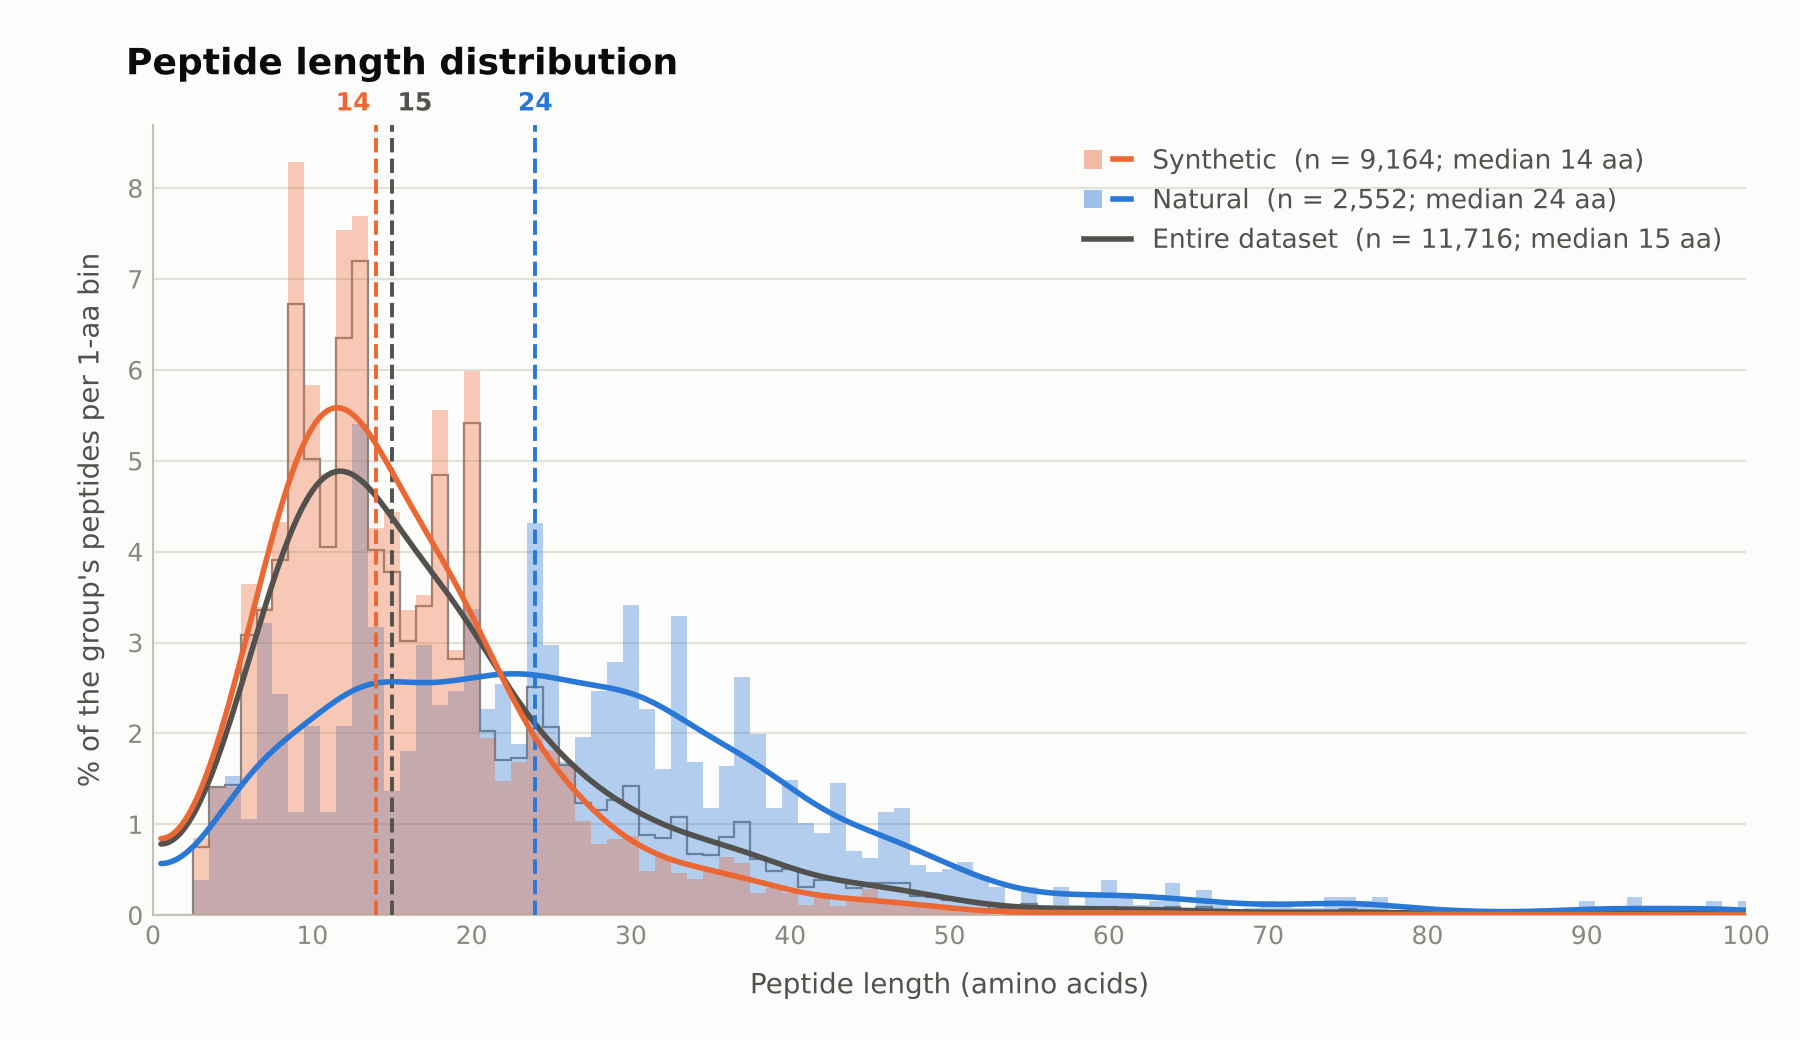
\includegraphics[width=0.92\textwidth]{deliverables/figures/length_histogram_overlap.png}
\caption{Length distribution, each group scaled to 100\,\% of itself; dashed lines = medians; curves = kernel densities.}
\end{figure}

\begin{table}[H]\centering\small
\begin{tabular}{lrrr}
\toprule
 & Natural & Synthetic & All\\\midrule
n & 2{,}552 & 9{,}164 & 11{,}716\\
median / mean (aa) & 24 / 26.9 & 14 / 16.0 & 15 / 18.4\\
Q1--Q3 (aa) & 14--35 & 10--20 & 10--23\\\midrule
Ultrashort 3--9\amin & 11.2\,\% & 23.3\,\% & \\
Short 10--24\amin & 39.2\,\% & \textbf{63.1\,\%} & \\
Medium 25--50\amin & \textbf{42.8\,\%} & 13.0\,\% & \\
Long 51--100\amin & 6.9\,\% & 0.6\,\% & \\\bottomrule
\end{tabular}
\caption{Length summary. Natural peptides make up 175 of the 232 Long peptides; Mann--Whitney $r=-0.46$, $p<10^{-270}$.}
\end{table}

\begin{itemize}
\item Natural peptides are longer: ribosomal host-defence peptides are typically 20--40 residues, and designers prefer short peptides (synthesis cost).
\item \textbf{The Synthetic histogram has spikes} (691 at 12\amin, 705 at 13 but 445 at 11; 549 at 20 but 267 at 19): design and library habits.
\item The short end of the Natural distribution is the \textbf{nonribosomal} peptides (median 7\amin).
\end{itemize}

%======================================================================
\section{Natural versus Synthetic: other annotations}
%======================================================================
\begin{table}[H]\centering\small
\begin{tabular}{lrrl}
\toprule
Property & Natural & Synthetic & chi-square\\\midrule
C-terminus modified (mostly amidation) & 22.8\,\% & \textbf{49.6\,\%} & $p\approx10^{-128}$\\
N-terminus modified (mostly acetylation) & 5.4\,\% & 7.7\,\% & $p\approx10^{-4}$, small\\
contains a D-amino acid & 5.6\,\% & 8.0\,\% & $p\approx10^{-4}$, small\\
contained \texttt{X} & 10.3\,\% & 9.9\,\% & $p=0.64$\\
tested vs Gram$-$ / Gram$+$ & 82 / 86\,\% & 79 / 76\,\% & similar focus\\
tested vs \textbf{fungi} & \textbf{52.2\,\%} & 21.6\,\% & $p\approx10^{-201}$\\
tested vs mammalian cells & 50.1\,\% & 55.7\,\% & small\\
target object: lipid bilayer & 85.2\,\% & 81.1\,\% & both membrane-active\\\bottomrule
\end{tabular}
\end{table}
(Source: \file{class_comparisons/overview/tables/annotation_tests_natural_vs_synthetic.csv}.)
C-terminal amidation removes the negative C-terminal charge and increases stability; designers use it routinely. D-amino acids, N-terminal modifications and non-standard residues
are concentrated in \textbf{nonribosomal} peptides (52\,\%, 37\,\% and 53\,\% of them), which is why they are common among bacterial and fungal peptides (Sect.~\ref{sec:cc}).

%======================================================================
\section{Amino acid enrichment: method}
%======================================================================
The official Composition Profiler \cite{vacic2007} (v2.0, \url{https://github.com/vvacic/cprofiler}) was used through its Python functions (the same as \texttt{cprof discover}).
Only the 20 single amino acids are tested (amino acid groups were dropped: they are sums of residues and the hydrophobicity scales disagreed), 10{,}000 permutations,
two-sided, Bonferroni $\alpha = 0.0025$, \texttt{np.random.seed(1)} before every test. The class comparisons use the same code; their Synthetic class reproduces the deliverable table exactly
(checked by the script).

\begin{table}[H]\centering\small
\begin{tabularx}{\textwidth}{>{\raggedright}p{2.4cm}>{\raggedright}p{5.6cm}X}
\toprule
Background & What it is & Question answered\tabularnewline\midrule
SwissProt & 5{,}002 proteins from SwissProt release 51 \cite{uniprot2023}, shipped with the tool; mean $\approx$360\amin; 1.8 million residues & How do AMPs differ from ordinary proteins?\tabularnewline
Non-AMP & 26{,}635 non-antimicrobial peptides from PepBench, 2--50\amin{} (median 18); 0.54 million residues & How do AMPs differ from short peptides that are not antimicrobial?\tabularnewline\bottomrule
\end{tabularx}
\end{table}

\begin{caution}[Limits of the backgrounds]
SwissProt release 51 (2006) sample of 5{,}002 proteins; the non-AMP set was used as supplied (its construction, e.g.\ matching by length or charge, was not audited; its high Lys/Arg content,
about 10\,\% each, suggests charge-matched negatives). Residues are pooled, so long peptides weigh more; there is no length adjustment.
\end{caution}

\paragraph{How to read a result.} Sign first, then size ($1+\text{effect}$ = fold change). ``$<0.0001$'' = no permutation reached the difference; ``not significant'' = $p>0.0025$.
Same sign and size in two groups = shared AMP feature; opposite sign = real difference. A residue enriched against both backgrounds is the most robust finding.
The scale is asymmetric (depletion stops at $-1$).

%======================================================================
\section{Amino acid enrichment: Natural versus Synthetic}
%======================================================================
\begin{figure}[H]\centering
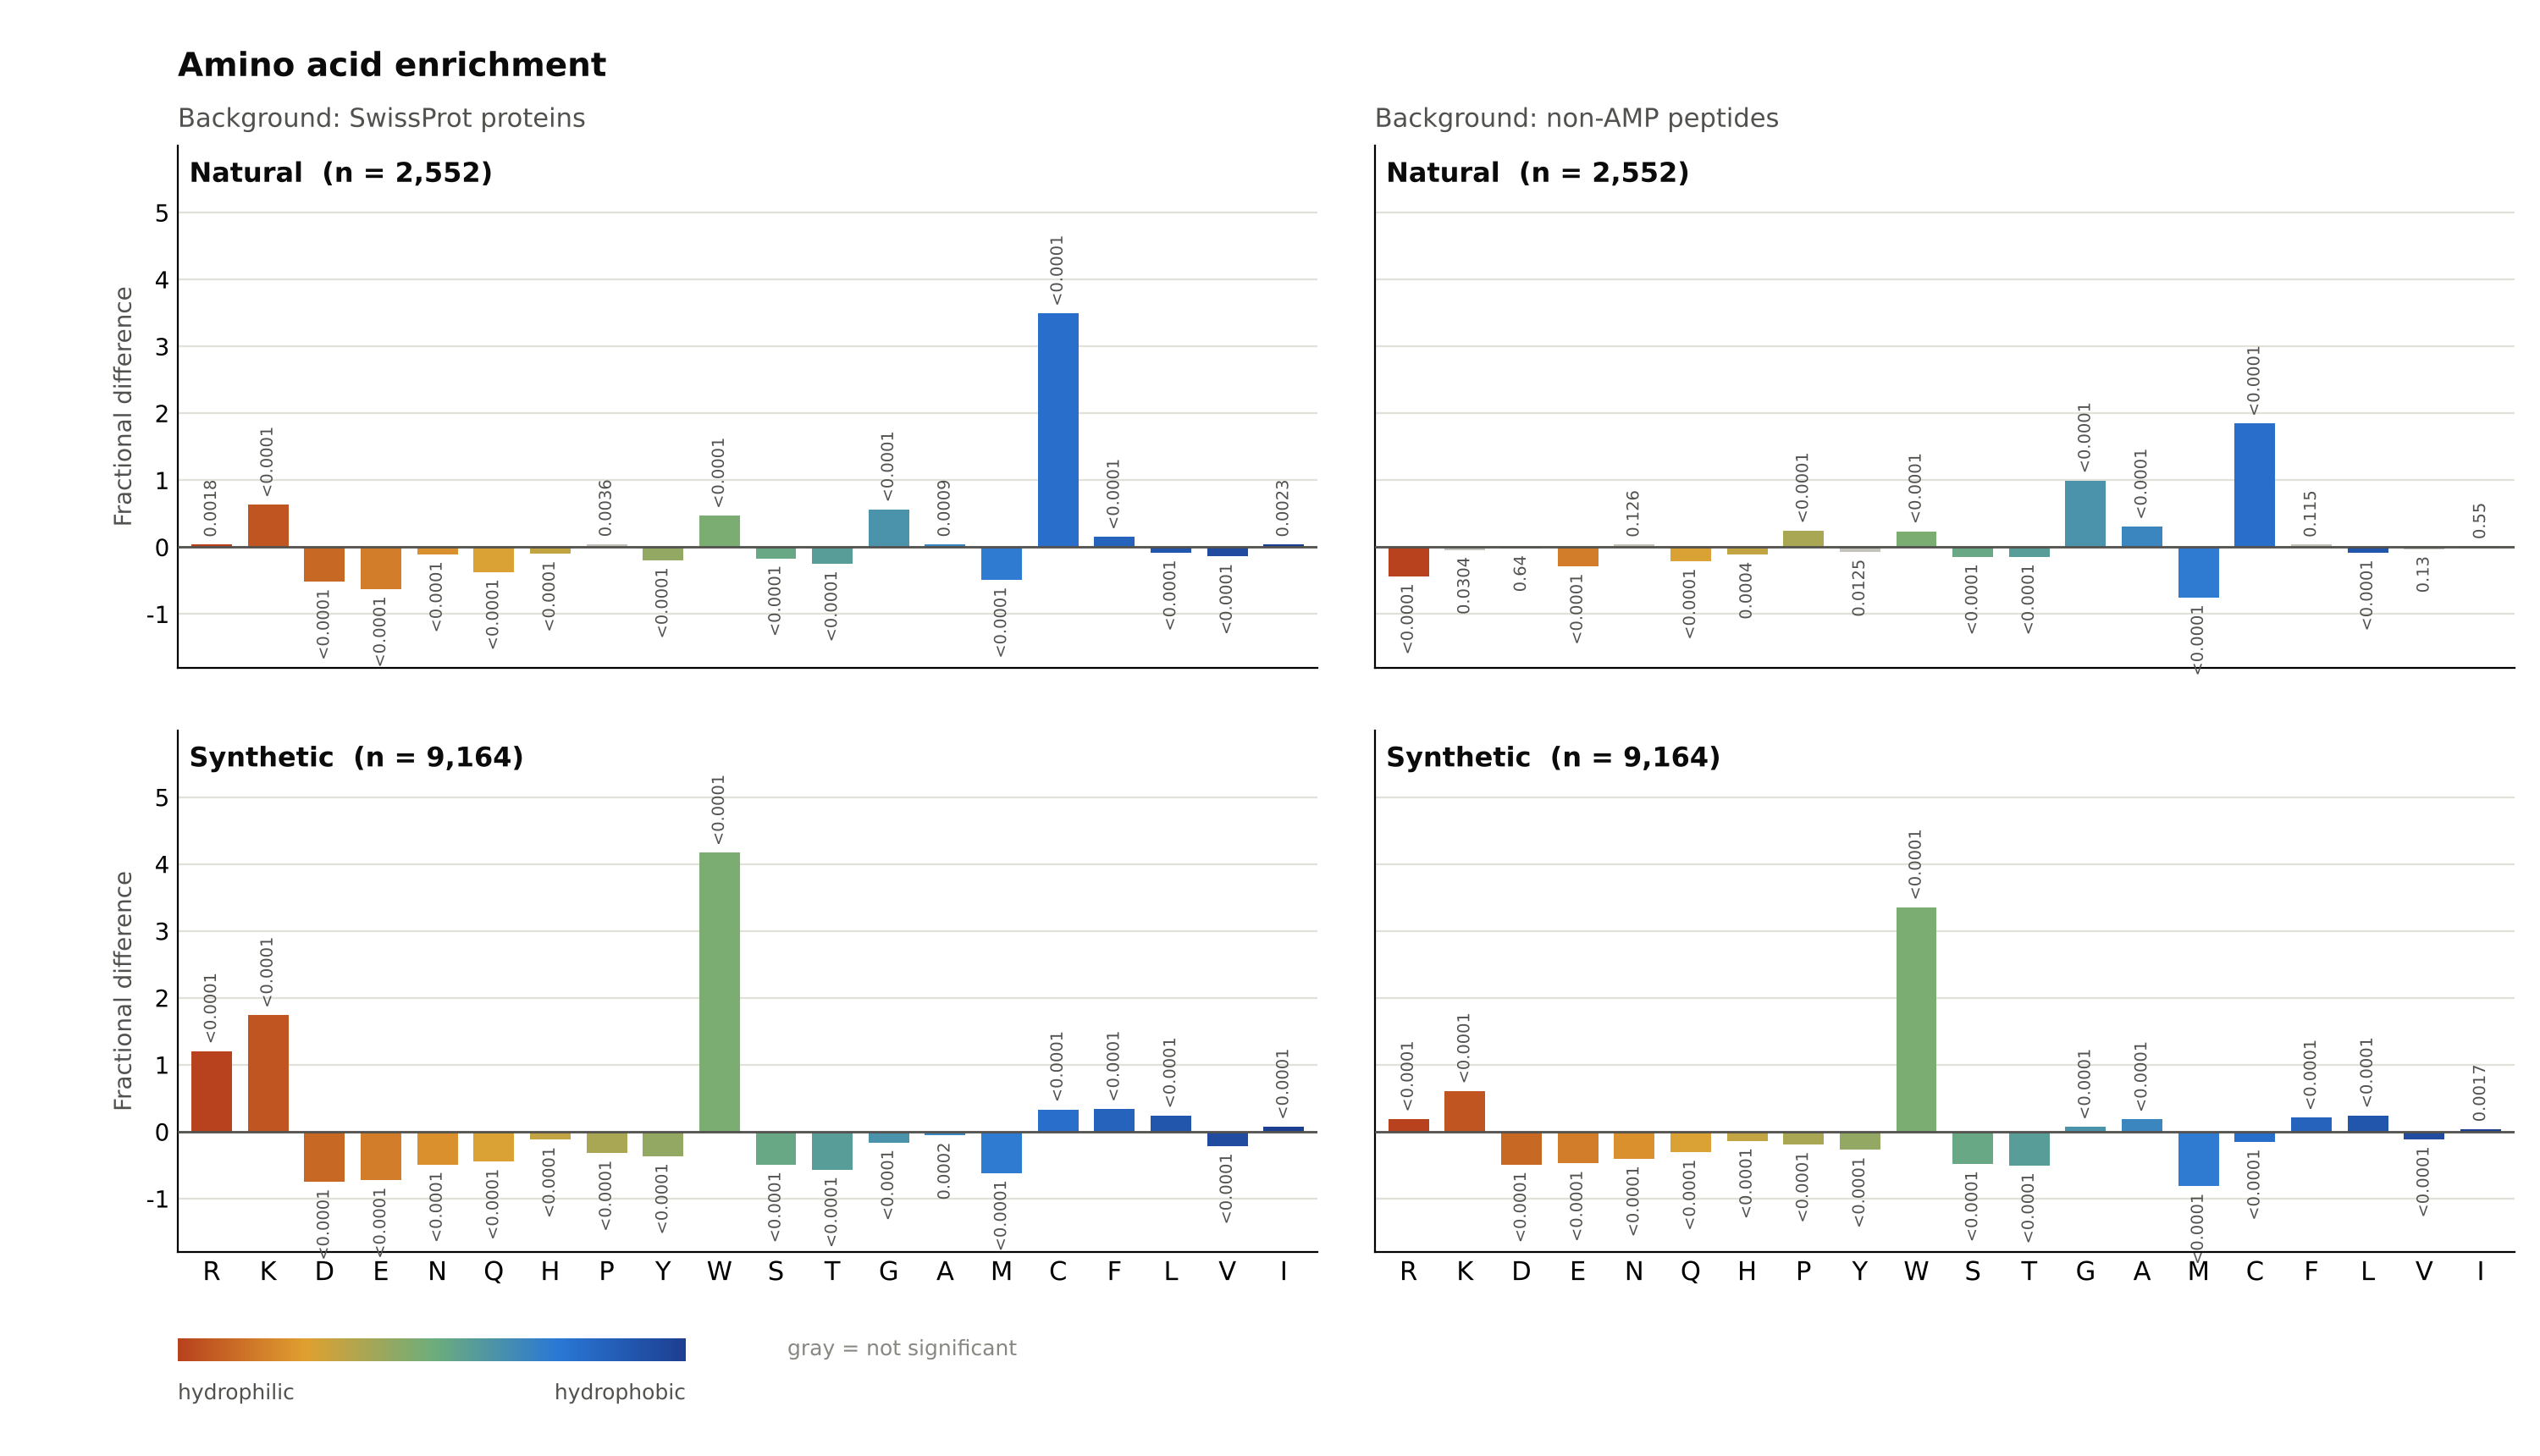
\includegraphics[width=\textwidth]{deliverables/figures/amino_acid_enrichment.png}
\caption{Fractional difference from the background, hydrophilic (R) to hydrophobic (I); numbers = p-values; grey = not significant.}
\end{figure}

\begin{table}[H]\centering\small
\begin{tabular}{crrrrrr}
\toprule
 & \multicolumn{2}{c}{Background, \% of residues} & \multicolumn{2}{c}{vs SwissProt} & \multicolumn{2}{c}{vs non-AMP}\\
\cmidrule(lr){2-3}\cmidrule(lr){4-5}\cmidrule(lr){6-7}
AA & SwissProt & non-AMP & Natural & Synthetic & Natural & Synthetic\\\midrule
R & 5.45 & 10.12 & $+0.04$ & $+1.20$ & $-0.44$ & $+0.19$\\
K & 5.96 & 10.15 & $+0.63$ & $+1.74$ & $-0.04$ ns & $+0.61$\\
D & 5.36 & 2.63 & $-0.52$ & $-0.75$ & $-0.02$ ns & $-0.49$\\
E & 6.68 & 3.49 & $-0.63$ & $-0.73$ & $-0.29$ & $-0.47$\\
N & 4.12 & 3.53 & $-0.11$ & $-0.49$ & $+0.04$ ns & $-0.40$\\
Q & 3.91 & 3.12 & $-0.37$ & $-0.45$ & $-0.21$ & $-0.31$\\
H & 2.30 & 2.34 & $-0.10$ & $-0.12$ & $-0.12$ & $-0.14$\\
P & 4.77 & 4.01 & $+0.05$ ns & $-0.32$ & $+0.25$ & $-0.19$\\
Y & 3.06 & 2.66 & $-0.20$ & $-0.37$ & $-0.08$ ns & $-0.27$\\
W & 1.15 & 1.36 & $+0.47$ & $\mathbf{+4.17}$ & $+0.24$ & $\mathbf{+3.35}$\\
S & 6.74 & 6.56 & $-0.17$ & $-0.49$ & $-0.15$ & $-0.48$\\
T & 5.32 & 4.68 & $-0.25$ & $-0.57$ & $-0.15$ & $-0.51$\\
G & 6.97 & 5.46 & $+0.56$ & $-0.16$ & $+1.00$ & $+0.07$\\
A & 7.91 & 6.33 & $+0.04$ & $-0.05$ & $+0.31$ & $+0.18$\\
M & 2.39 & 4.95 & $-0.49$ & $-0.62$ & $-0.75$ & $-0.82$\\
C & 1.50 & 2.36 & $\mathbf{+3.49}$ & $+0.33$ & $\mathbf{+1.85}$ & $-0.16$\\
F & 3.98 & 4.41 & $+0.15$ & $+0.34$ & $+0.04$ ns & $+0.21$\\
L & 9.71 & 9.70 & $-0.09$ & $+0.24$ & $-0.08$ & $+0.24$\\
V & 6.76 & 5.99 & $-0.14$ & $-0.22$ & $-0.03$ ns & $-0.11$\\
I & 5.98 & 6.16 & $+0.04$ & $+0.07$ & $+0.01$ ns & $+0.04$\\\bottomrule
\end{tabular}
\caption{Fractional differences (ns = not significant after Bonferroni). Source: \texttt{deliverables/tables/aa\_enrichment.csv}.}
\end{table}

\begin{enumerate}
\item \textbf{Against proteins, both groups look like AMPs}: more K, R, W; much less D, E, M, Q, T, S.
\item \textbf{Synthetic peptides exaggerate the recipe}: Trp $\times5.2$, Lys $\times2.7$, Arg $\times2.2$; Natural peptides go the same way gently (Lys $\times1.6$, Trp $\times1.5$, Arg unchanged).
\item \textbf{Natural peptides carry Cys and Gly}: Cys $\times4.5$, Gly $\times1.6$ (disulfide-rich, defensin-like folds).
\item \textbf{Against non-AMP peptides} (Lys/Arg-rich themselves), Natural peptides have less Arg and equal Lys; what remains distinctive is Trp in Synthetic ($+3.35$), Cys ($+1.85$) and Gly ($+1.00$)
      in Natural, and low Met in both.
\item \textbf{Opposite directions} (real origin differences): Gly, Pro, Leu (vs SwissProt), Cys (vs non-AMP).
\end{enumerate}

%======================================================================
\section{Class comparisons}\label{sec:cc}
%======================================================================
\subsection{Design}
\file{class_comparisons/scripts/01-05} attach class labels to the 11{,}716 peptides and repeat the deliverable analysis for every class with at least 50 peptides.
Each comparison folder has, in \file{figures/}: \textbf{length\_histogram\_overlap.png} (one panel per class, class in blue vs the whole population in grey, as \% of the group,
with medians; same bins and smoothing as the deliverable), its counts version, \textbf{length\_category\_fraction\_bar.png} (100\,\% stacked length categories; first bar = population),
\textbf{amino\_acid\_enrichment.png} (one row per class $\times$ both backgrounds, identical axes; bars above $+5$ are cut and their value written in the bar) and
\textbf{enrichment\_heatmap.png} (same numbers, compact). Tables: length summary, categories, tests (Mann--Whitney vs the rest of the population with $r$; Kruskal--Wallis where classes do not overlap)
and the enrichment table; \file{fasta/} holds each class's peptides.

\begin{table}[H]\centering\small
\begin{tabularx}{\textwidth}{>{\raggedright}p{3.0cm}>{\raggedright}p{8.4cm}X}
\toprule
Comparison & Tested classes ($n\geq50$) & Not tested\tabularnewline\midrule
Source organism (Natural) & Animalia 1{,}789; Bacteria 396; Plantae 266; Fungi 73 & Unclassified 21, Archaea 3, Protista 2, two kingdoms 2\tabularnewline
Synthesis type & Ribosomal 2{,}301; Nonribosomal 251; Synthetic 9{,}164 & \tabularnewline
Function (all) & Gram$-$ 9{,}353; Gram$+$ 9{,}160; mammalian cell 6{,}385; antifungal 3{,}316; anticancer 2{,}189; antiviral 747; antibiofilm 356; antiparasitic 219; insecticidal 60 & antiprotozoal 33, nematicidal 28, anti-mollicute 18\tabularnewline
Function (Natural) & Gram$+$ 2{,}192; Gram$-$ 2{,}104; antifungal 1{,}332; mammalian cell 1{,}279; anticancer 538; antiparasitic 129; antiviral 112; antibiofilm 53 & insecticidal 37, \dots\tabularnewline
Target object & lipid bilayer 9{,}606; virus entry 342; cytoplasmic protein 176; DNA/RNA 158; virus replication 152; membrane protein 115; virus integrase 104; Lipid II 81; virus protease 59; ribosome 59 & 14 smaller objects\tabularnewline\bottomrule
\end{tabularx}
\caption{Classes and sizes (\texttt{class\_comparisons/overview/tables/class\_sizes.csv}).}
\end{table}

\begin{caution}[Three facts that shape the class comparisons]
\begin{enumerate}
\item \textbf{Function and target-object classes overlap}: median 3 target groups per peptide; Jaccard 0.83 between the two antibacterial classes and 0.53--0.57 with mammalian-cell testing.
\item \textbf{Synthetic peptides are 78\,\%} of the data, so ``function (all)'' and ``target object'' mostly show the synthetic composition; ``function (Natural)'' is the fairer test.
\item \textbf{\texttt{X}$\rightarrow$Ala inflates Ala unevenly} (Table~\ref{tab:xshare}): in nonribosomal and Lipid II peptides about one residue in ten was \texttt{X}; their Ala enrichment is not a finding.
\end{enumerate}
\end{caution}

\begin{table}[H]\centering\small
\begin{tabular}{lrr}
\toprule
Class & peptides with former \texttt{X} & former \texttt{X}, \% of residues\\\midrule
Nonribosomal & 52.6\,\% & 10.4\,\%\\
Lipid II (target object) & 80.2\,\% & 9.9\,\%\\
Membrane protein (target object) & 44.3\,\% & 5.4\,\%\\
Ribosome (target object) & 39.0\,\% & 4.0\,\%\\
Bacteria & 39.9\,\% & 3.8\,\%\\
Fungi & 27.4\,\% & 1.7\,\%\\
all other classes & & $\leq 1.4$\,\%\\\bottomrule
\end{tabular}
\caption{How much Ala is inflated by the cleaning, per class (\texttt{former\_x\_share\_by\_class.csv}).}
\label{tab:xshare}
\end{table}

\subsection{Source organism (Natural peptides)}
\begin{figure}[H]\centering
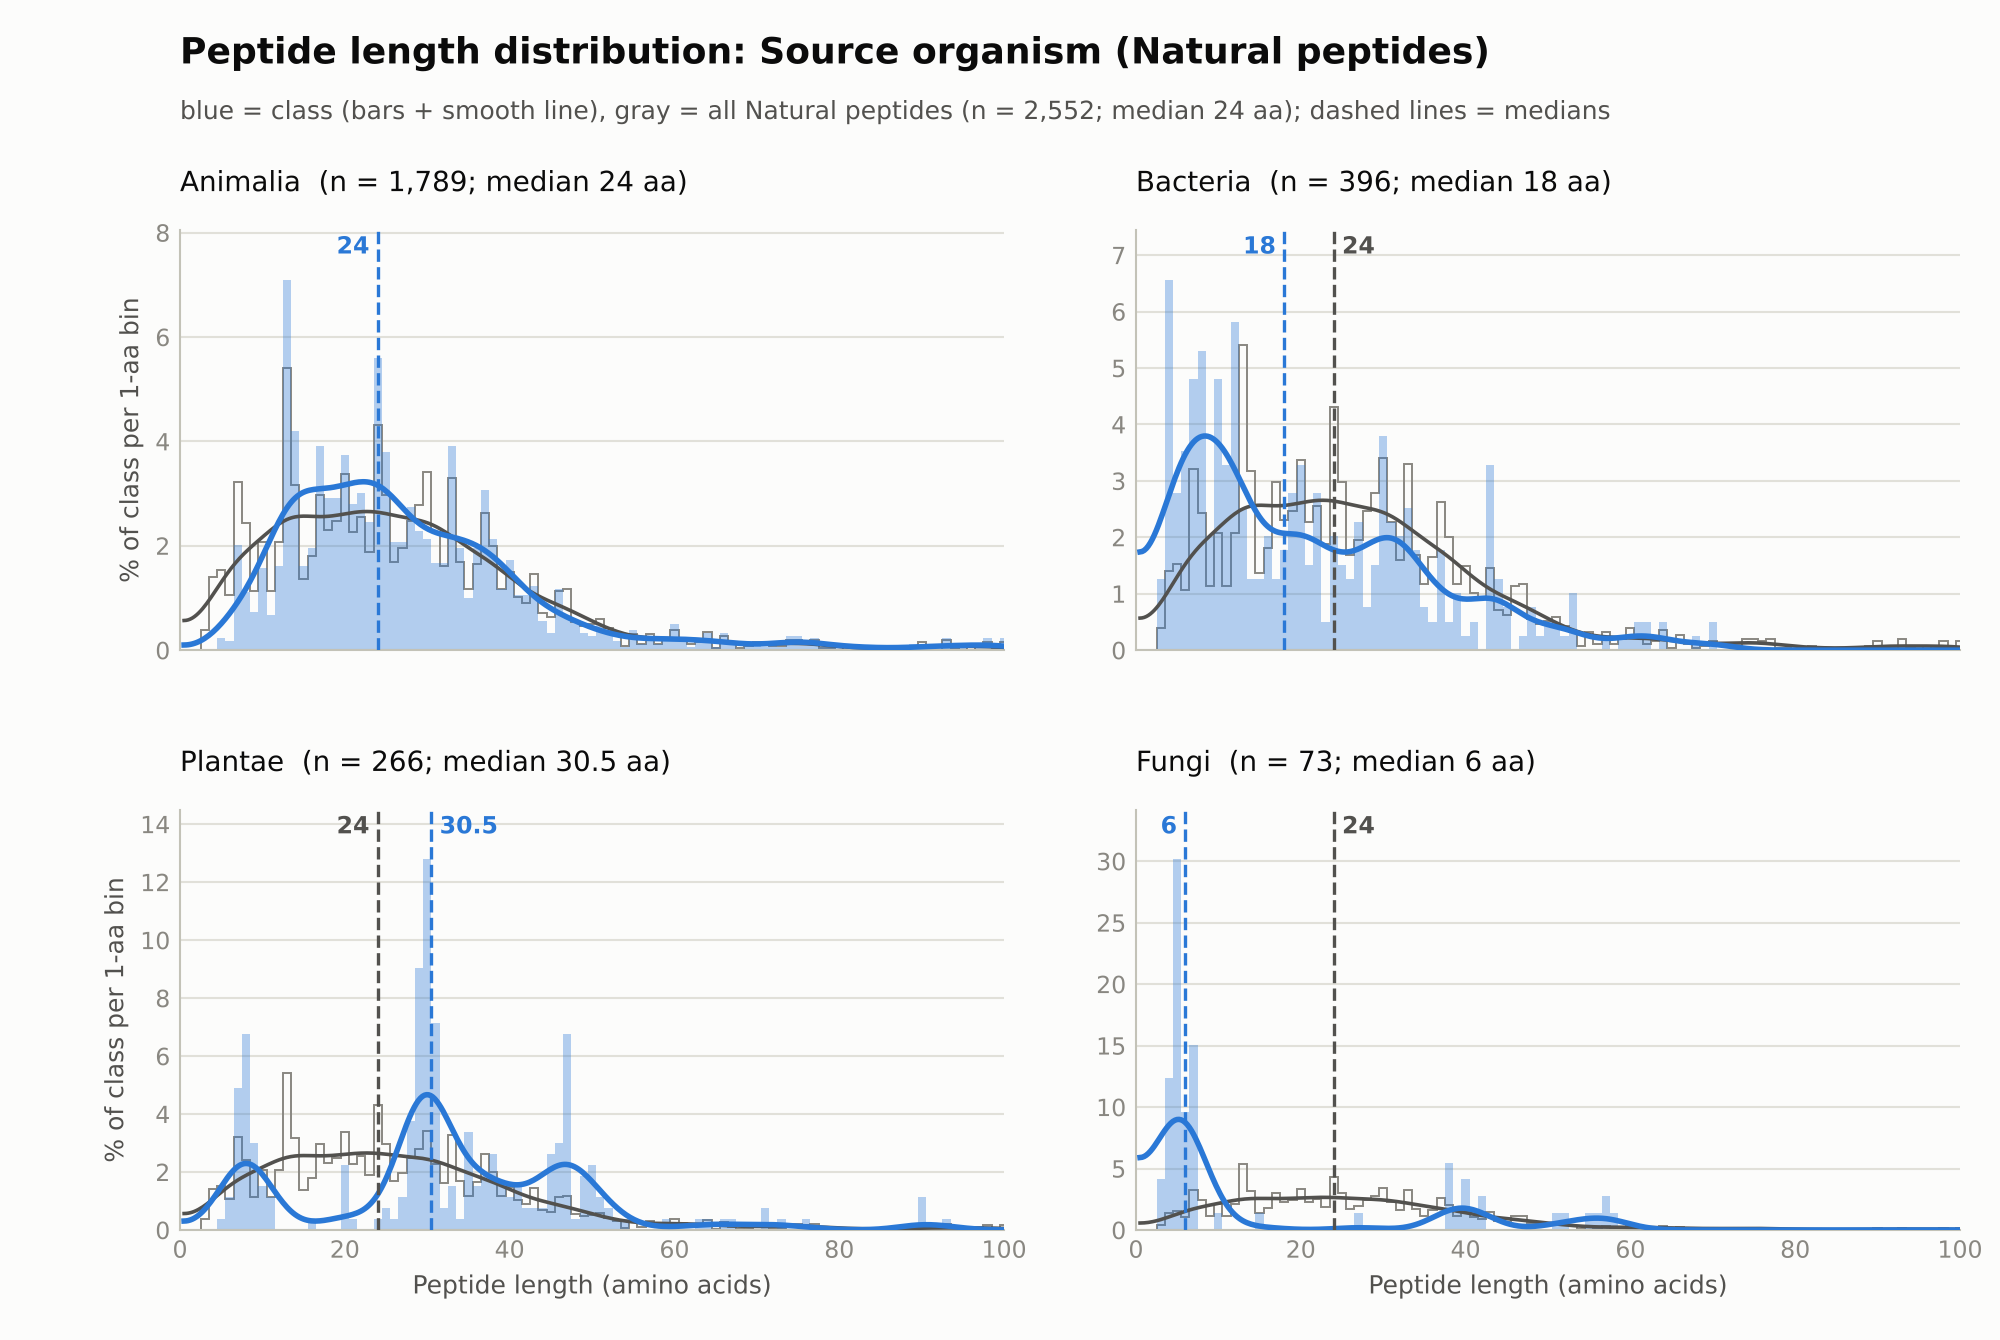
\includegraphics[width=0.9\textwidth]{class_comparisons/source_organism/figures/length_histogram_overlap.png}
\caption{Length by source organism (blue) against all Natural peptides (grey).}
\end{figure}
\begin{figure}[H]\centering
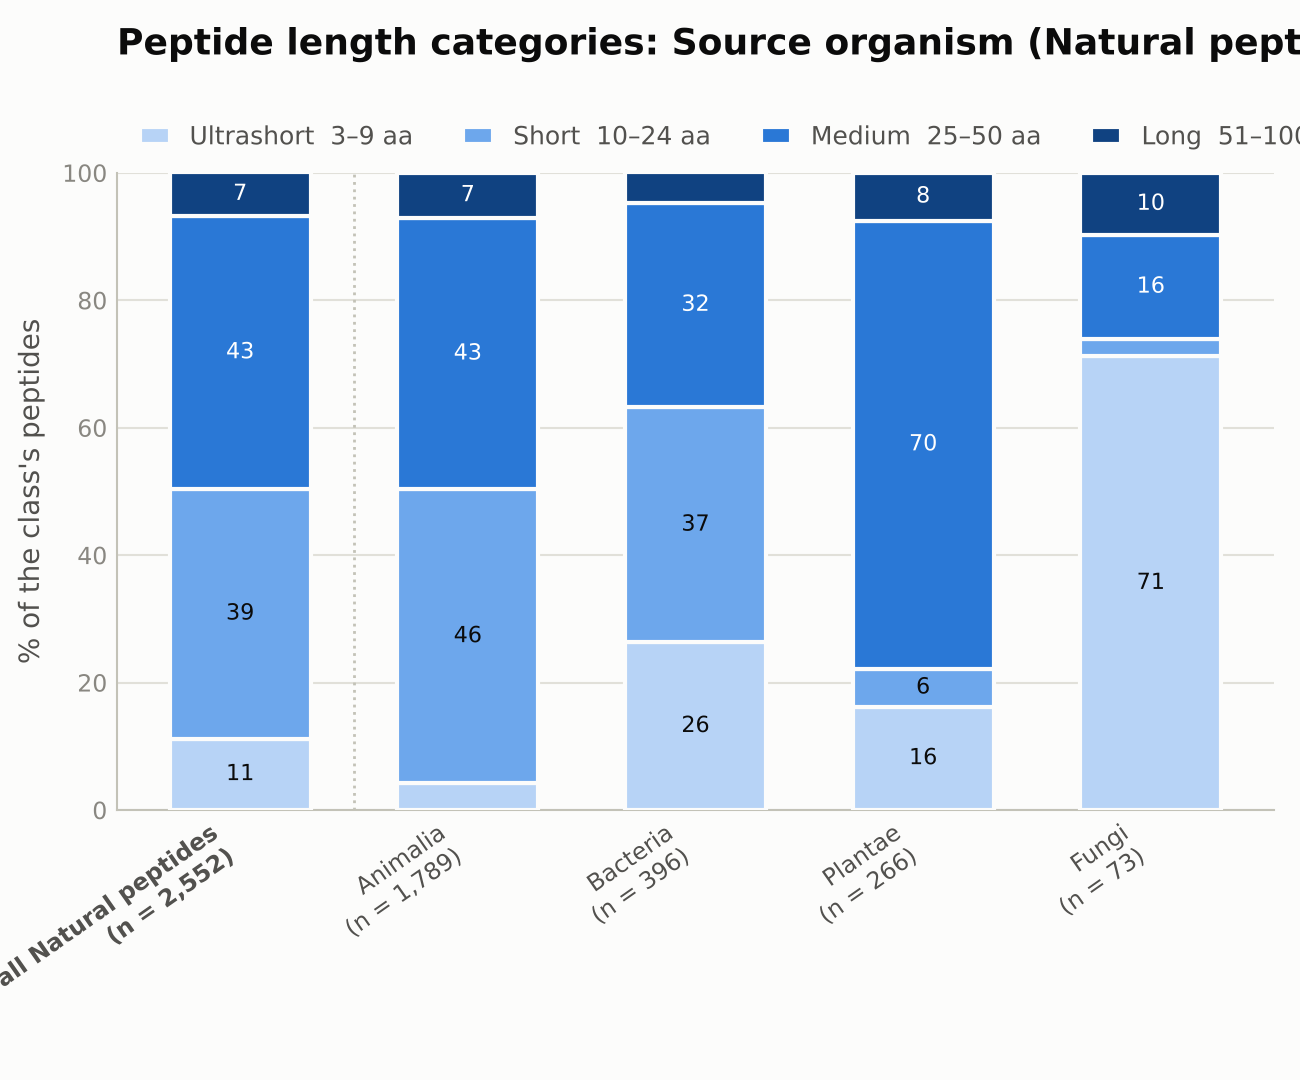
\includegraphics[width=0.62\textwidth]{class_comparisons/source_organism/figures/length_category_fraction_bar.png}
\caption{Length categories by source organism (first bar = all Natural peptides).}
\end{figure}
\begin{figure}[H]\centering
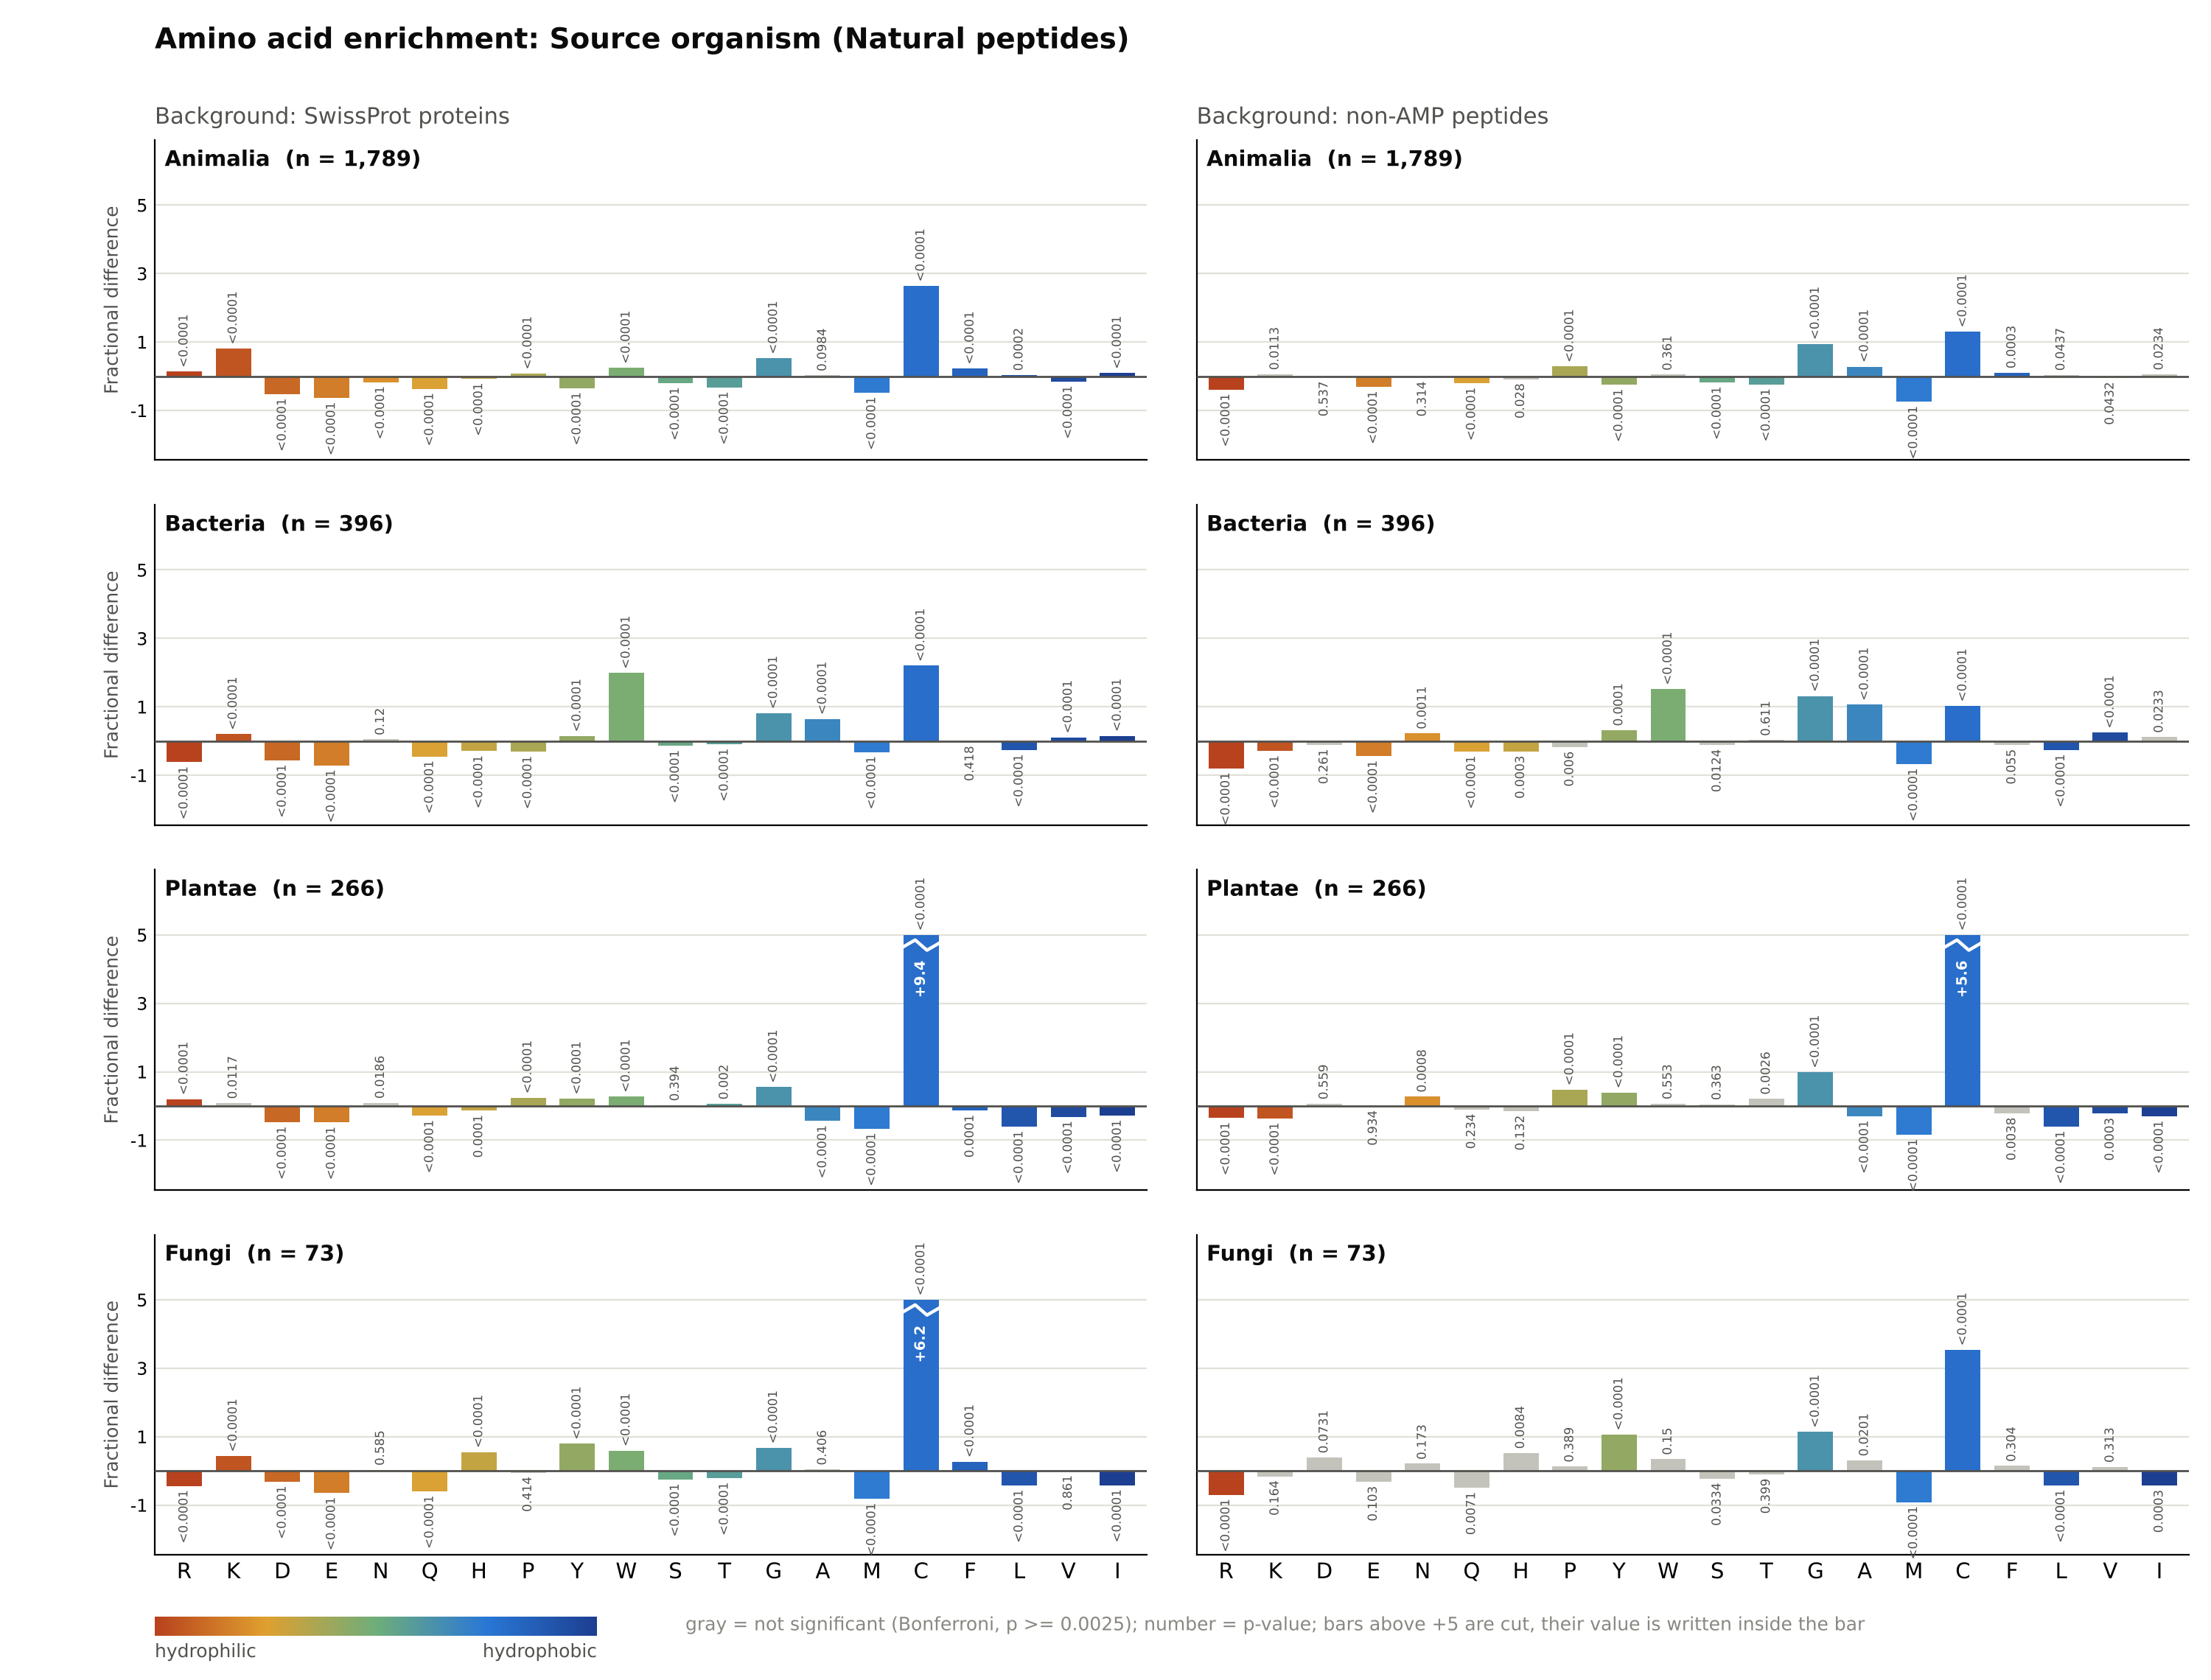
\includegraphics[width=\textwidth]{class_comparisons/source_organism/figures/amino_acid_enrichment.png}
\caption{Enrichment by source organism.}
\end{figure}

\begin{table}[H]\centering\footnotesize\setlength{\tabcolsep}{3pt}
\resizebox{\textwidth}{!}{%
\begin{tabular}{lrrrrrrr}
\toprule
\% vs SwissProt (non-AMP) & median & Cys & Gly & Trp & Lys & Arg & Met\\\midrule
Animalia (1{,}789) & 24 & $+264$ ($+131$) & $+52$ ($+95$) & $+24$ ($+5$ ns) & $+81$ ($+6$ ns) & $+13$ ($-39$) & $-48$ ($-75$)\\
Bacteria (396) & 18 & $+220$ ($+103$) & $+82$ ($+132$) & $\mathbf{+199}$ ($+152$) & $+20$ ($-29$) & $-62$ ($-79$) & $-32$ ($-67$)\\
Plantae (266) & 30.5 & $\mathbf{+937}$ ($+557$) & $+55$ ($+98$) & $+27$ ($+7$ ns) & $+9$ ns ($-36$) & $+20$ ($-35$) & $-66$ ($-84$)\\
Fungi (73) & 6 & $\mathbf{+616}$ ($+354$) & $+67$ ($+114$) & $+60$ ($+34$ ns) & $+43$ ($-16$ ns) & $-44$ ($-70$) & $-82$ ($-91$)\\\bottomrule
\end{tabular}}
\end{table}
\begin{itemize}
\item \textbf{One natural signature in every kingdom}: Cys and Gly up, Met, Glu, Gln down, against both backgrounds. Plants and fungi are the most Cys-rich.
\item \textbf{Length}: Plantae are longest (70\,\% are 25--50\amin), Fungi shortest (71\,\% are 3--9\amin; $r=-0.51$), Bacteria short (26\,\% ultrashort); Kruskal--Wallis $p=10^{-36}$.
\item Bacterial and fungal peptides often carry D-amino acids (25\,\% / 48\,\%), N-terminal modifications (22\,\% / 30\,\%) and former \texttt{X} (40\,\% / 27\,\%): many are nonribosomal products.
\item Against non-AMP peptides the natural classes are \emph{not} cationic: Arg is depleted in all four and Lys is not enriched.
\end{itemize}

\subsection{Synthesis type}
\begin{figure}[H]\centering
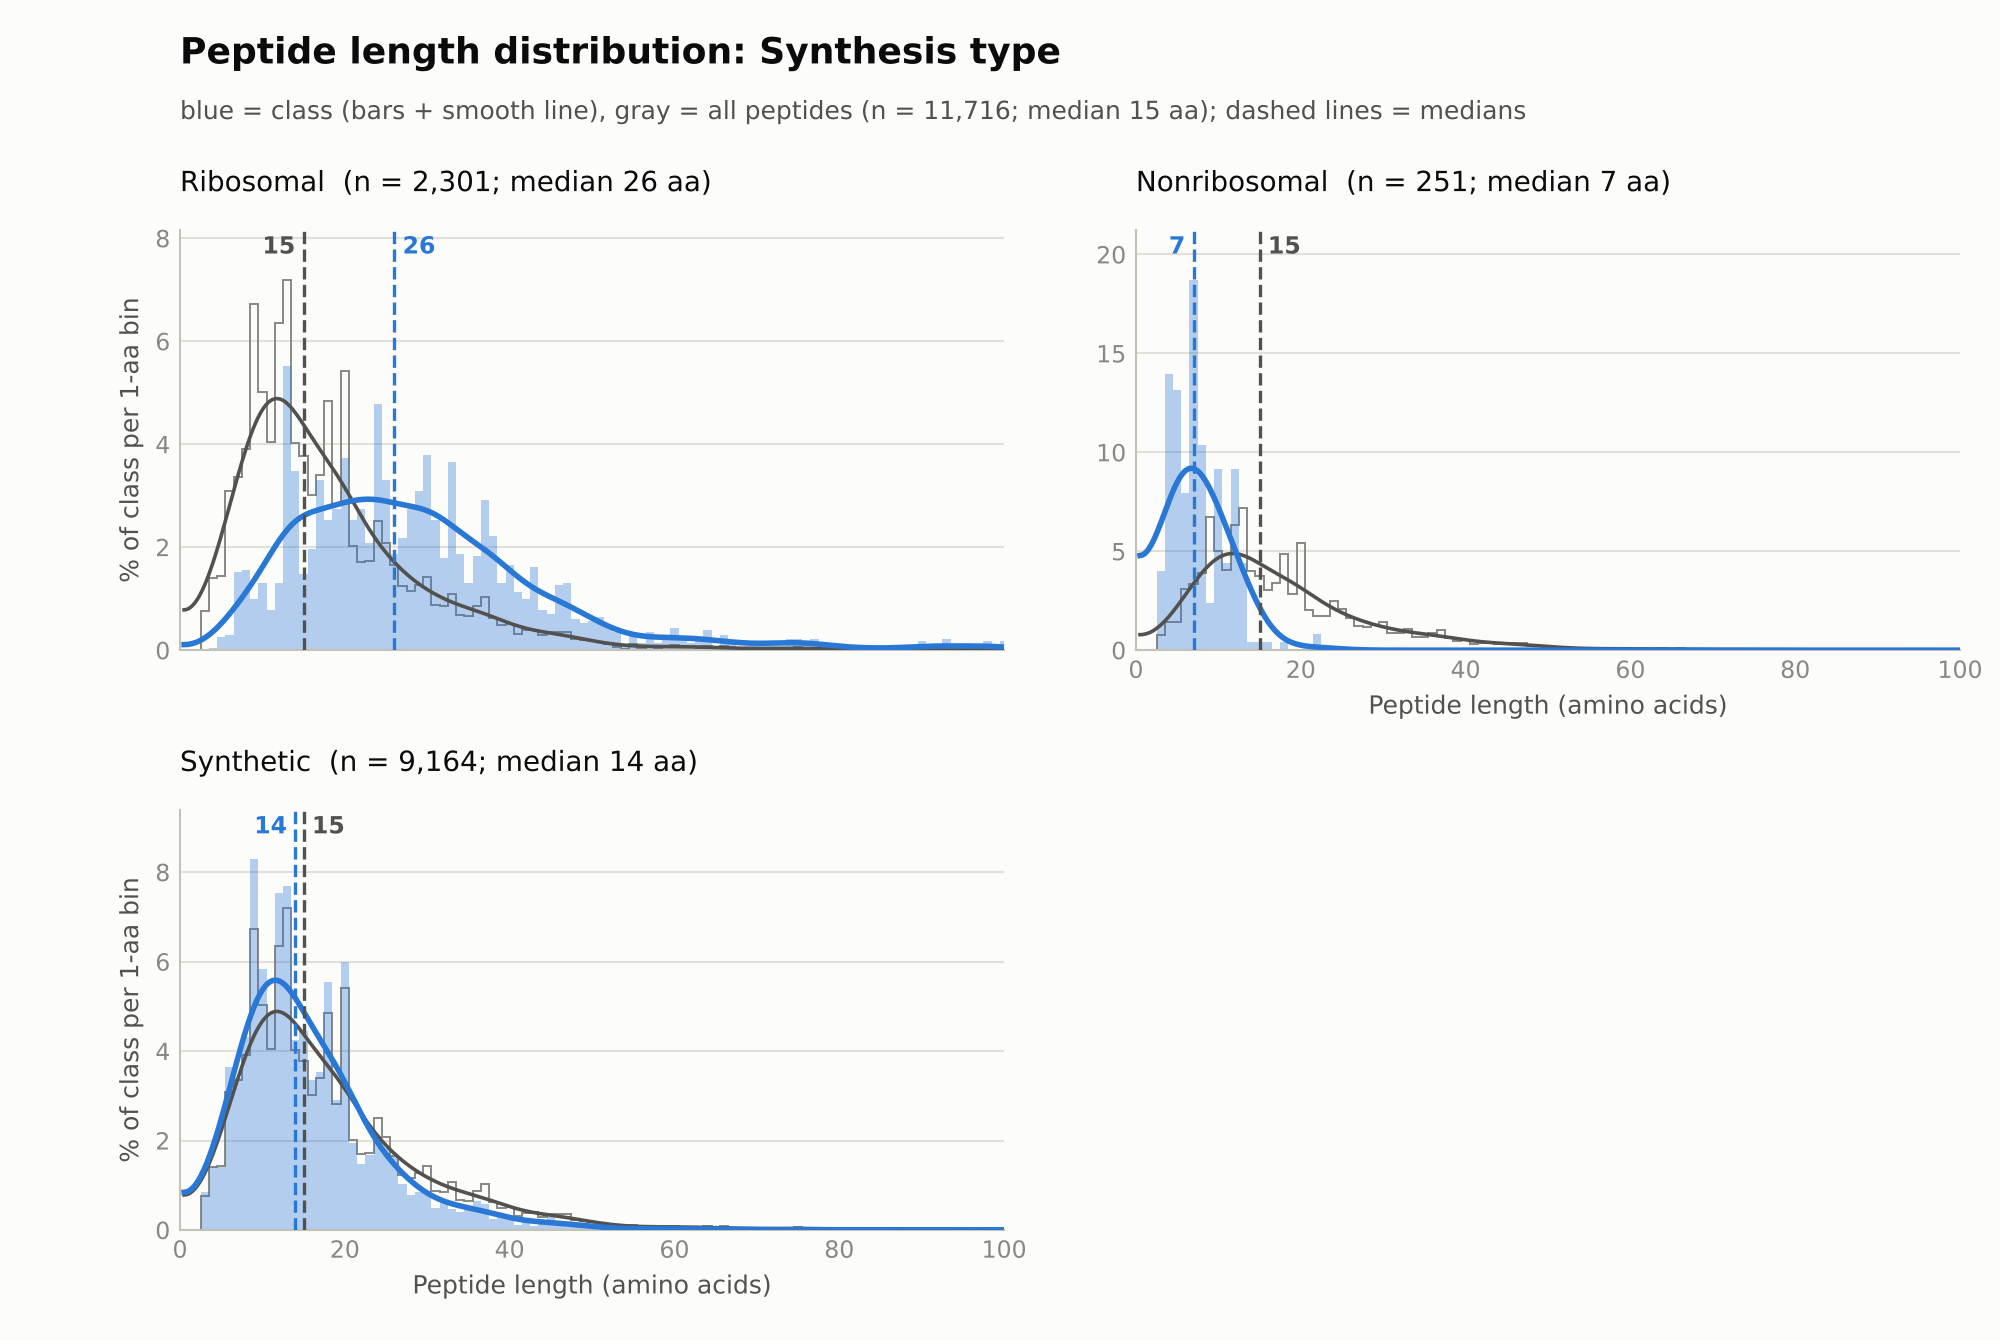
\includegraphics[width=0.85\textwidth]{class_comparisons/synthesis_type/figures/length_histogram_overlap.png}
\caption{Length by synthesis type (blue) against all peptides (grey).}
\end{figure}
\begin{figure}[H]\centering
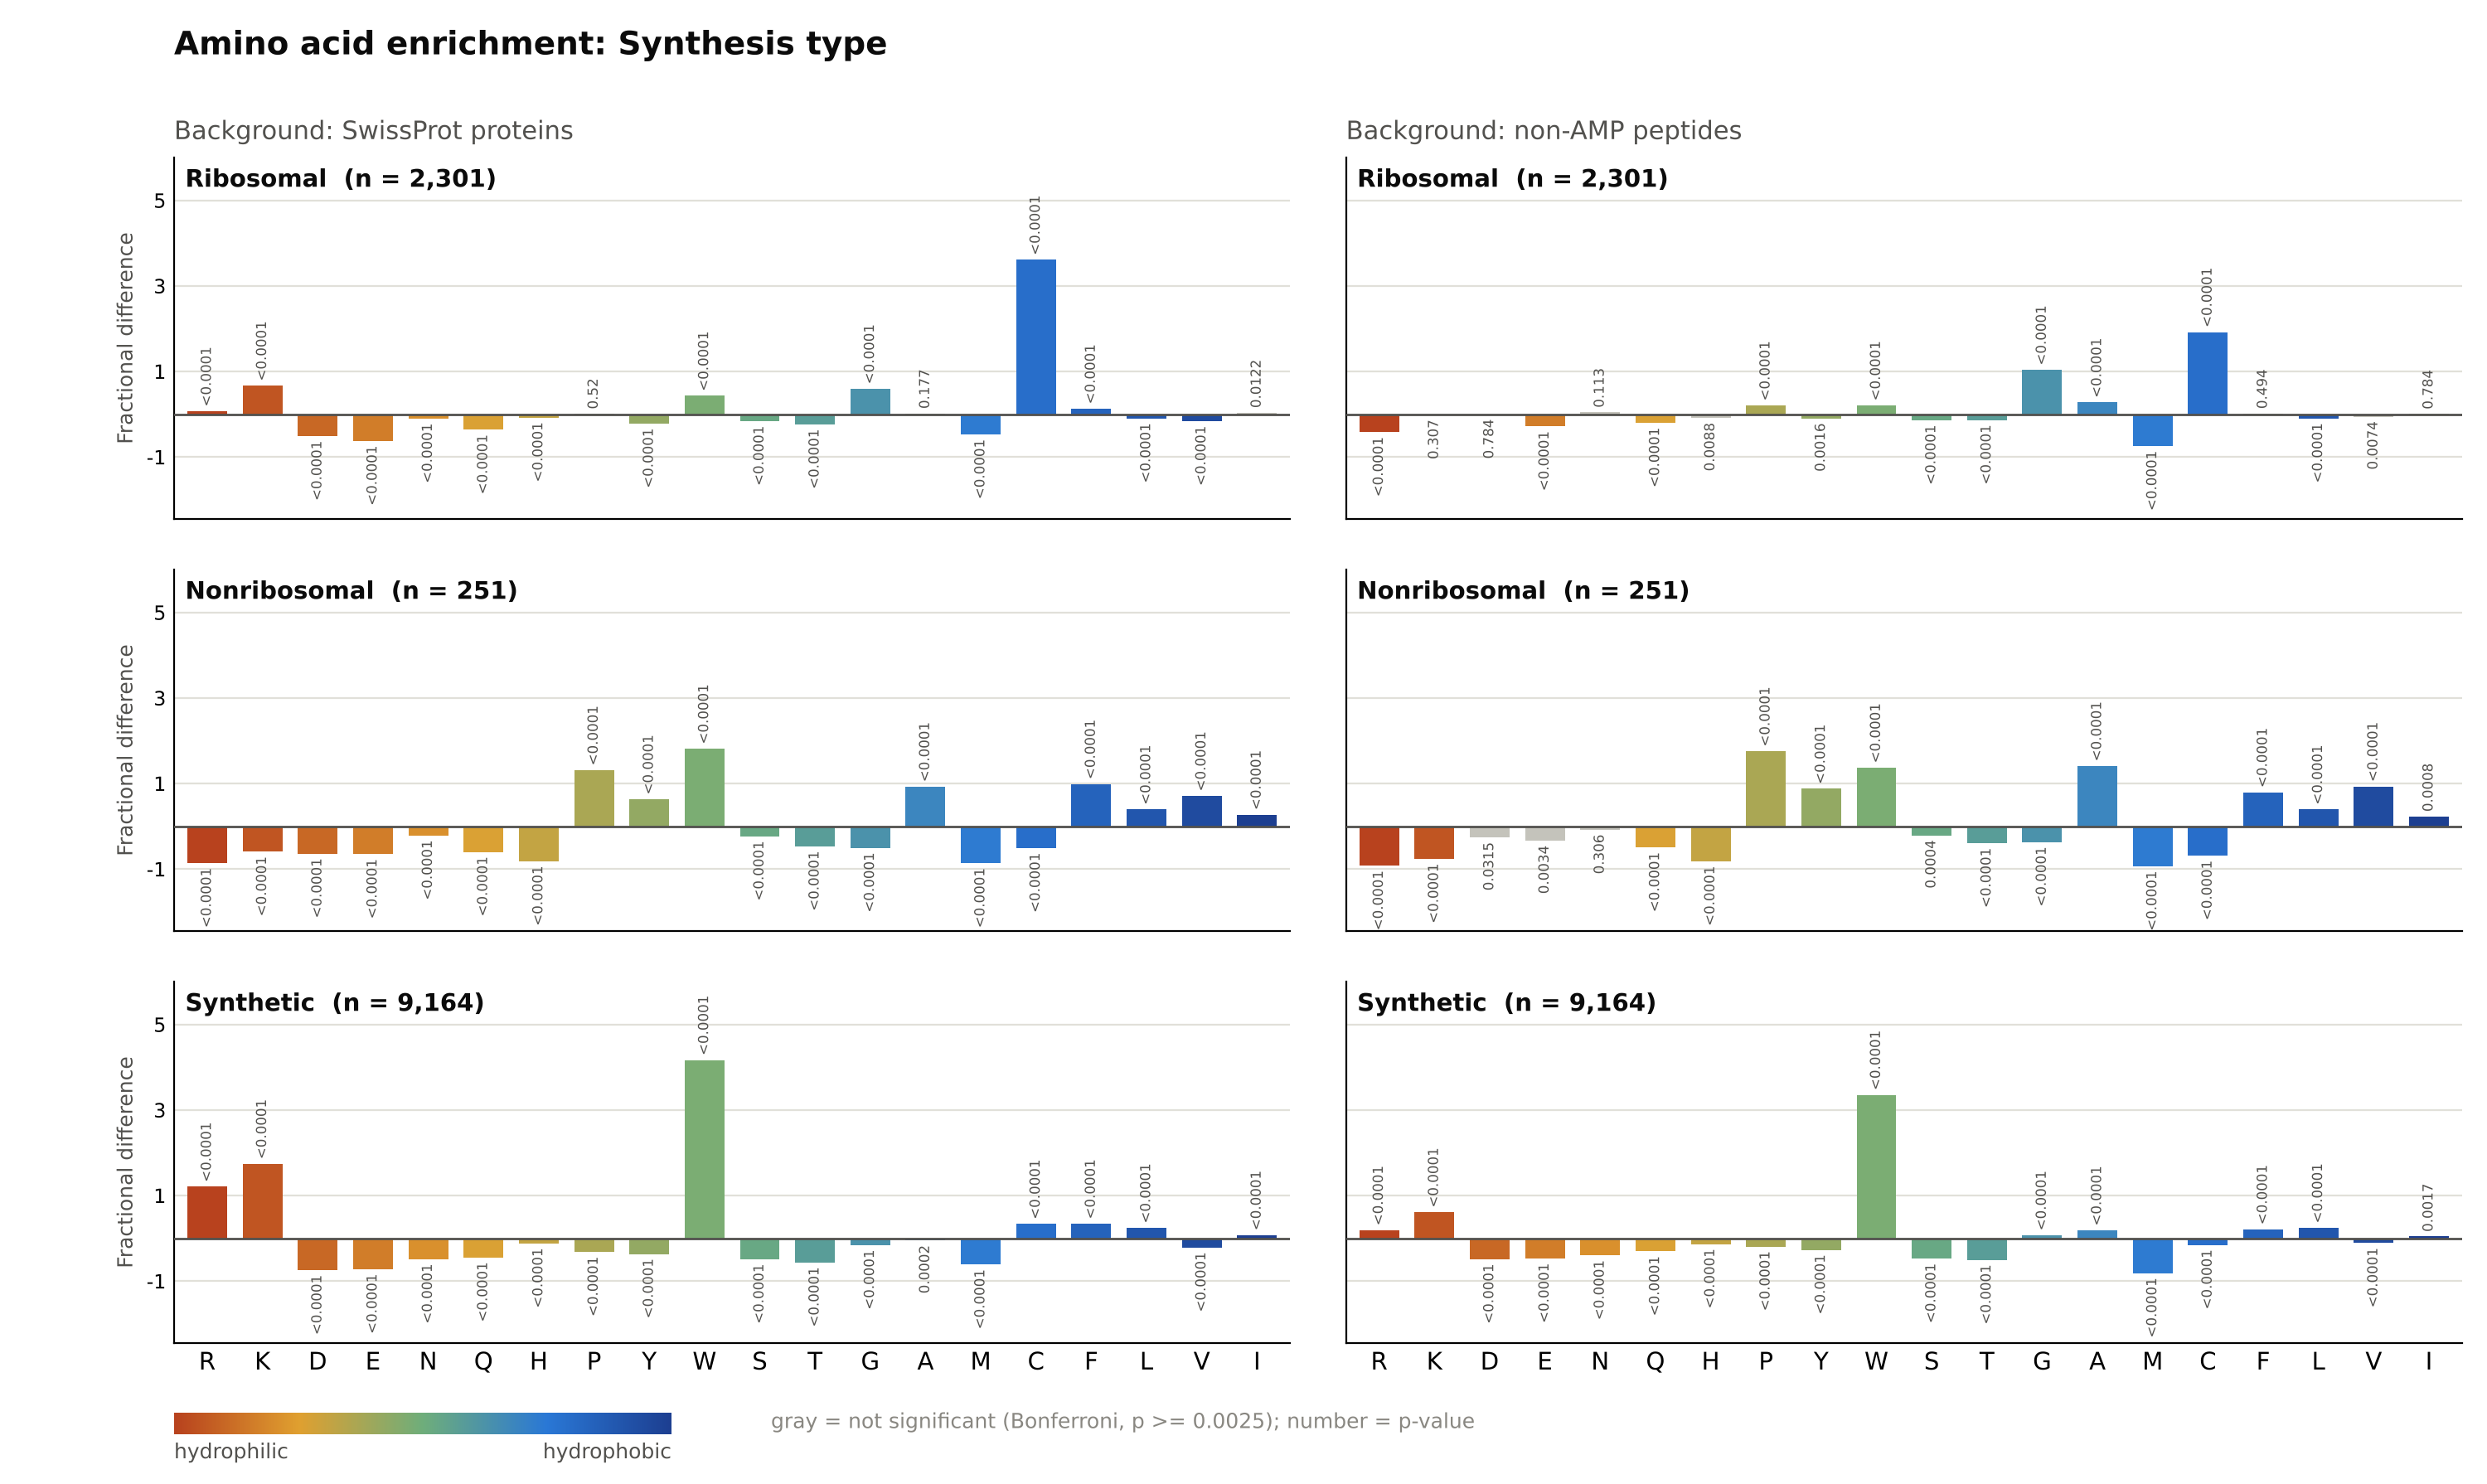
\includegraphics[width=\textwidth]{class_comparisons/synthesis_type/figures/amino_acid_enrichment.png}
\caption{Enrichment by synthesis type.}
\end{figure}
\begin{itemize}
\item \textbf{Ribosomal} (median 26\amin): the natural signature (Cys $+361$\,\%, Gly $+59$\,\%, Lys $+67$\,\%).
\item \textbf{Nonribosomal} (median 7\amin, none above 22, $r=-0.74$): Pro $+131$\,\%, Trp $+181$\,\%, Phe $+99$\,\%, Val $+71$\,\%, Tyr $+63$\,\%; Arg $-87$\,\%, Lys $-60$\,\%, Met $-87$\,\%, Cys $-51$\,\%.
      Short, aromatic/Pro-rich and not cationic. (Their Ala $+93$\,\% comes from \texttt{X}.)
\item \textbf{Synthetic}: Trp $+417$\,\%, Lys $+174$\,\%, Arg $+121$\,\%, little Cys.
\end{itemize}

\subsection{Function (target group)}
\begin{figure}[H]\centering
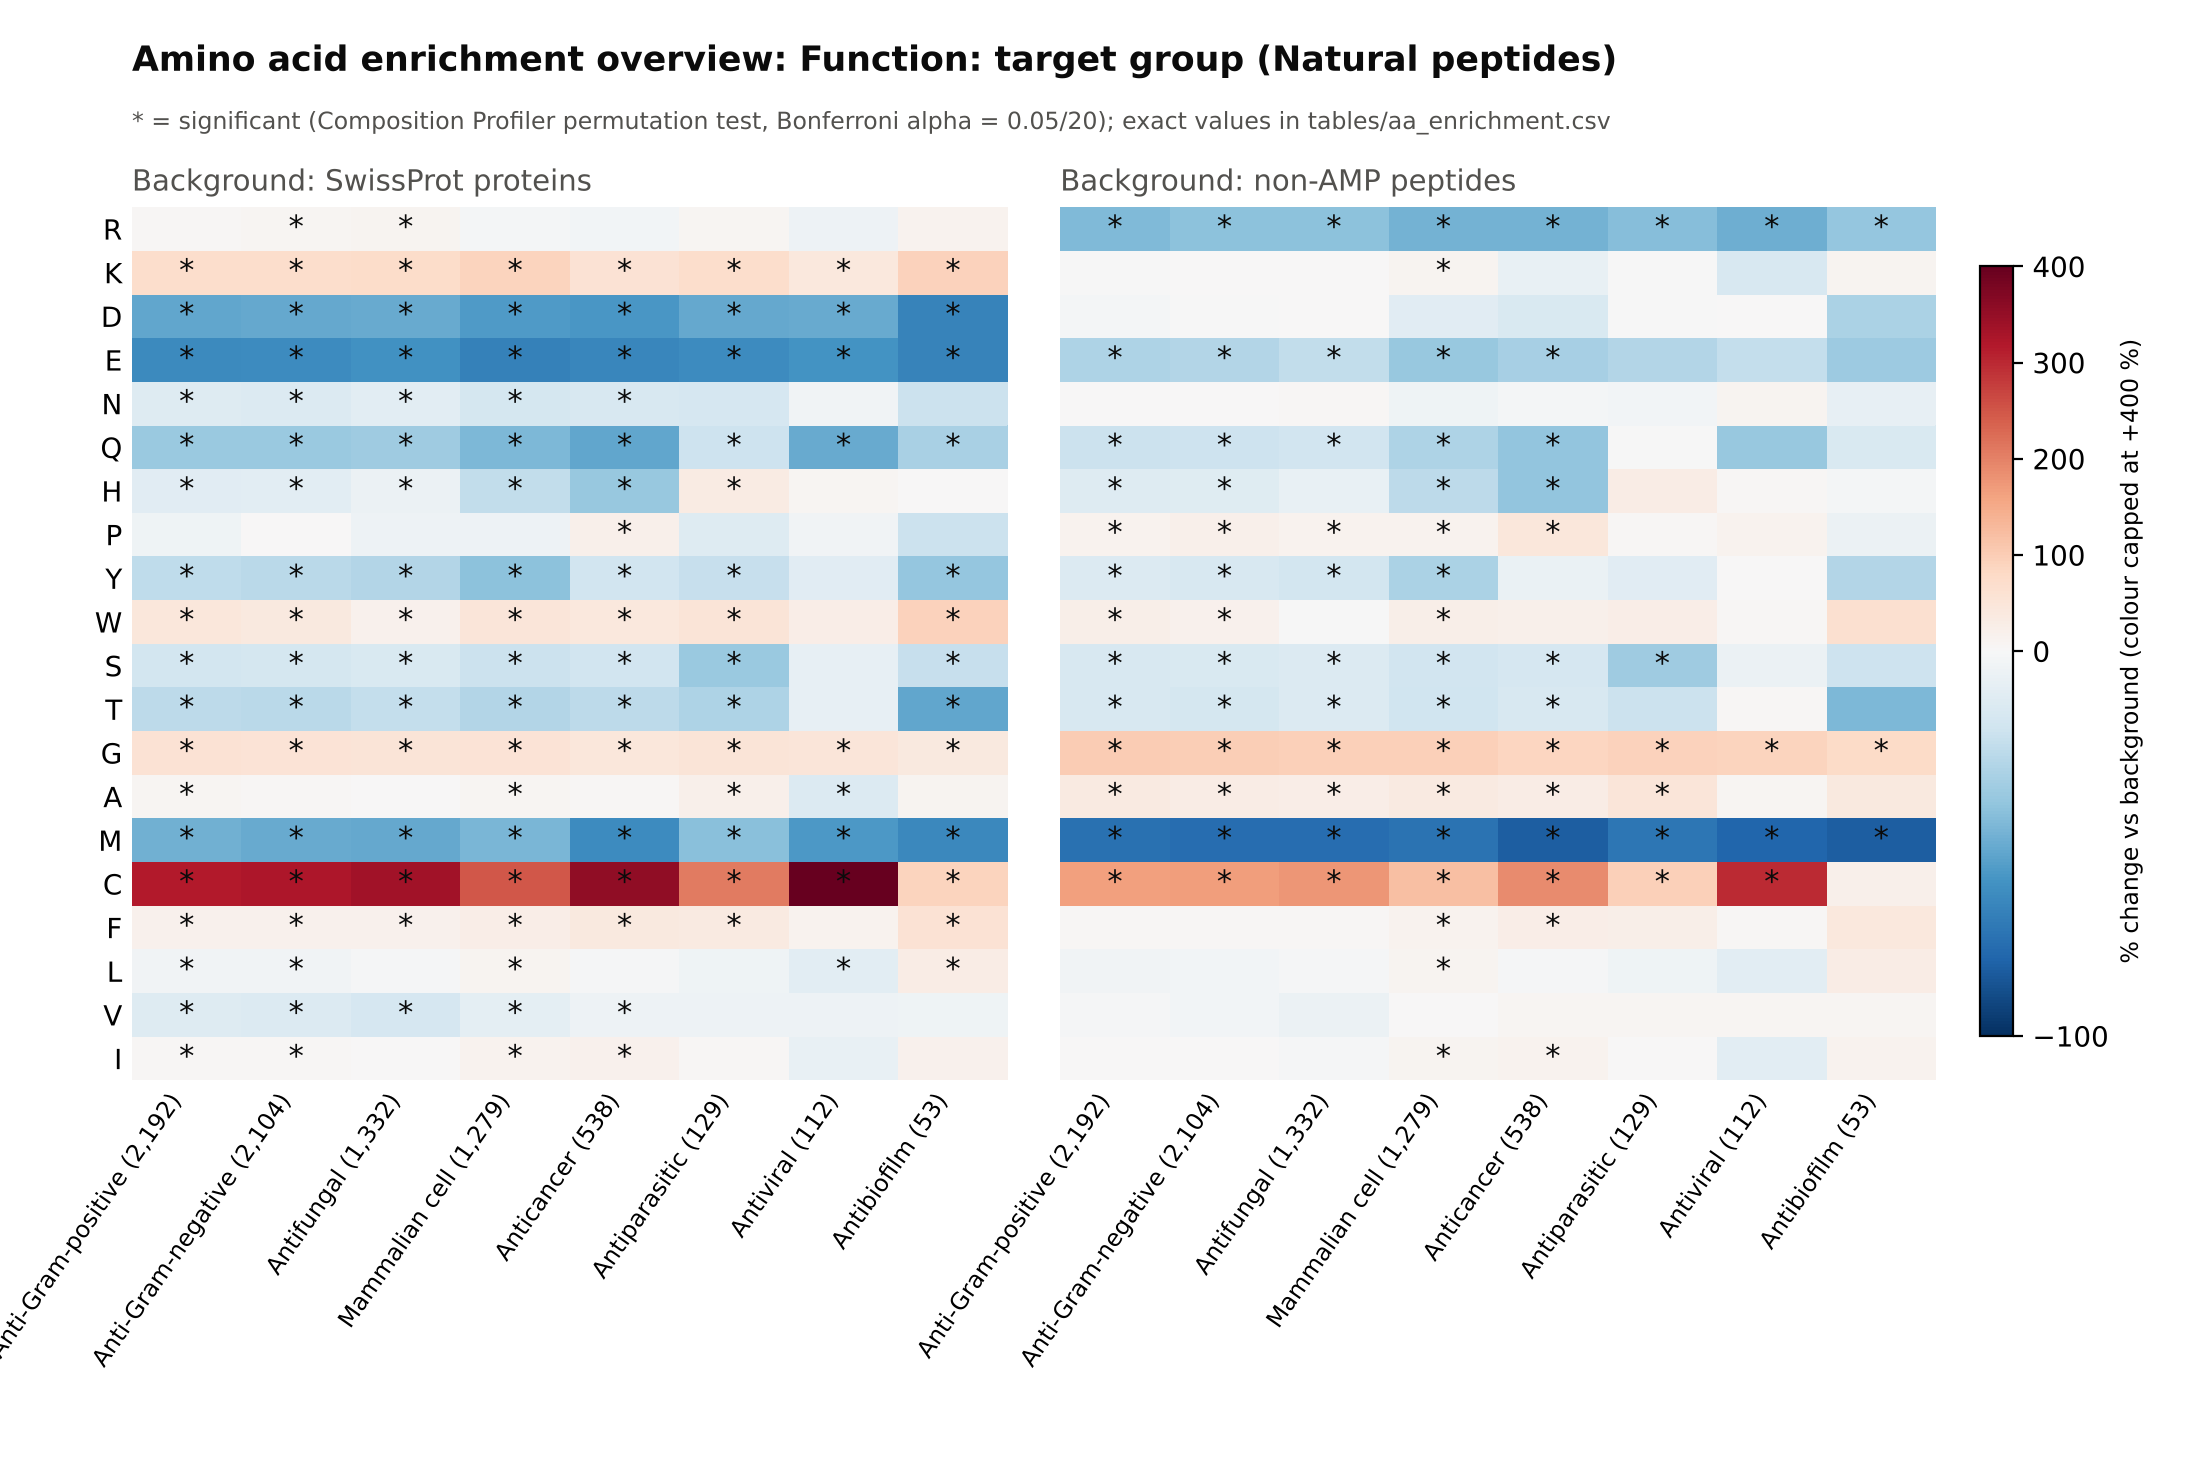
\includegraphics[width=\textwidth]{class_comparisons/function_natural/figures/enrichment_heatmap.png}
\caption{Enrichment of Natural peptides by target group (heatmap view; the bar view is \texttt{amino\_acid\_enrichment.png}).}
\end{figure}
\begin{figure}[H]\centering
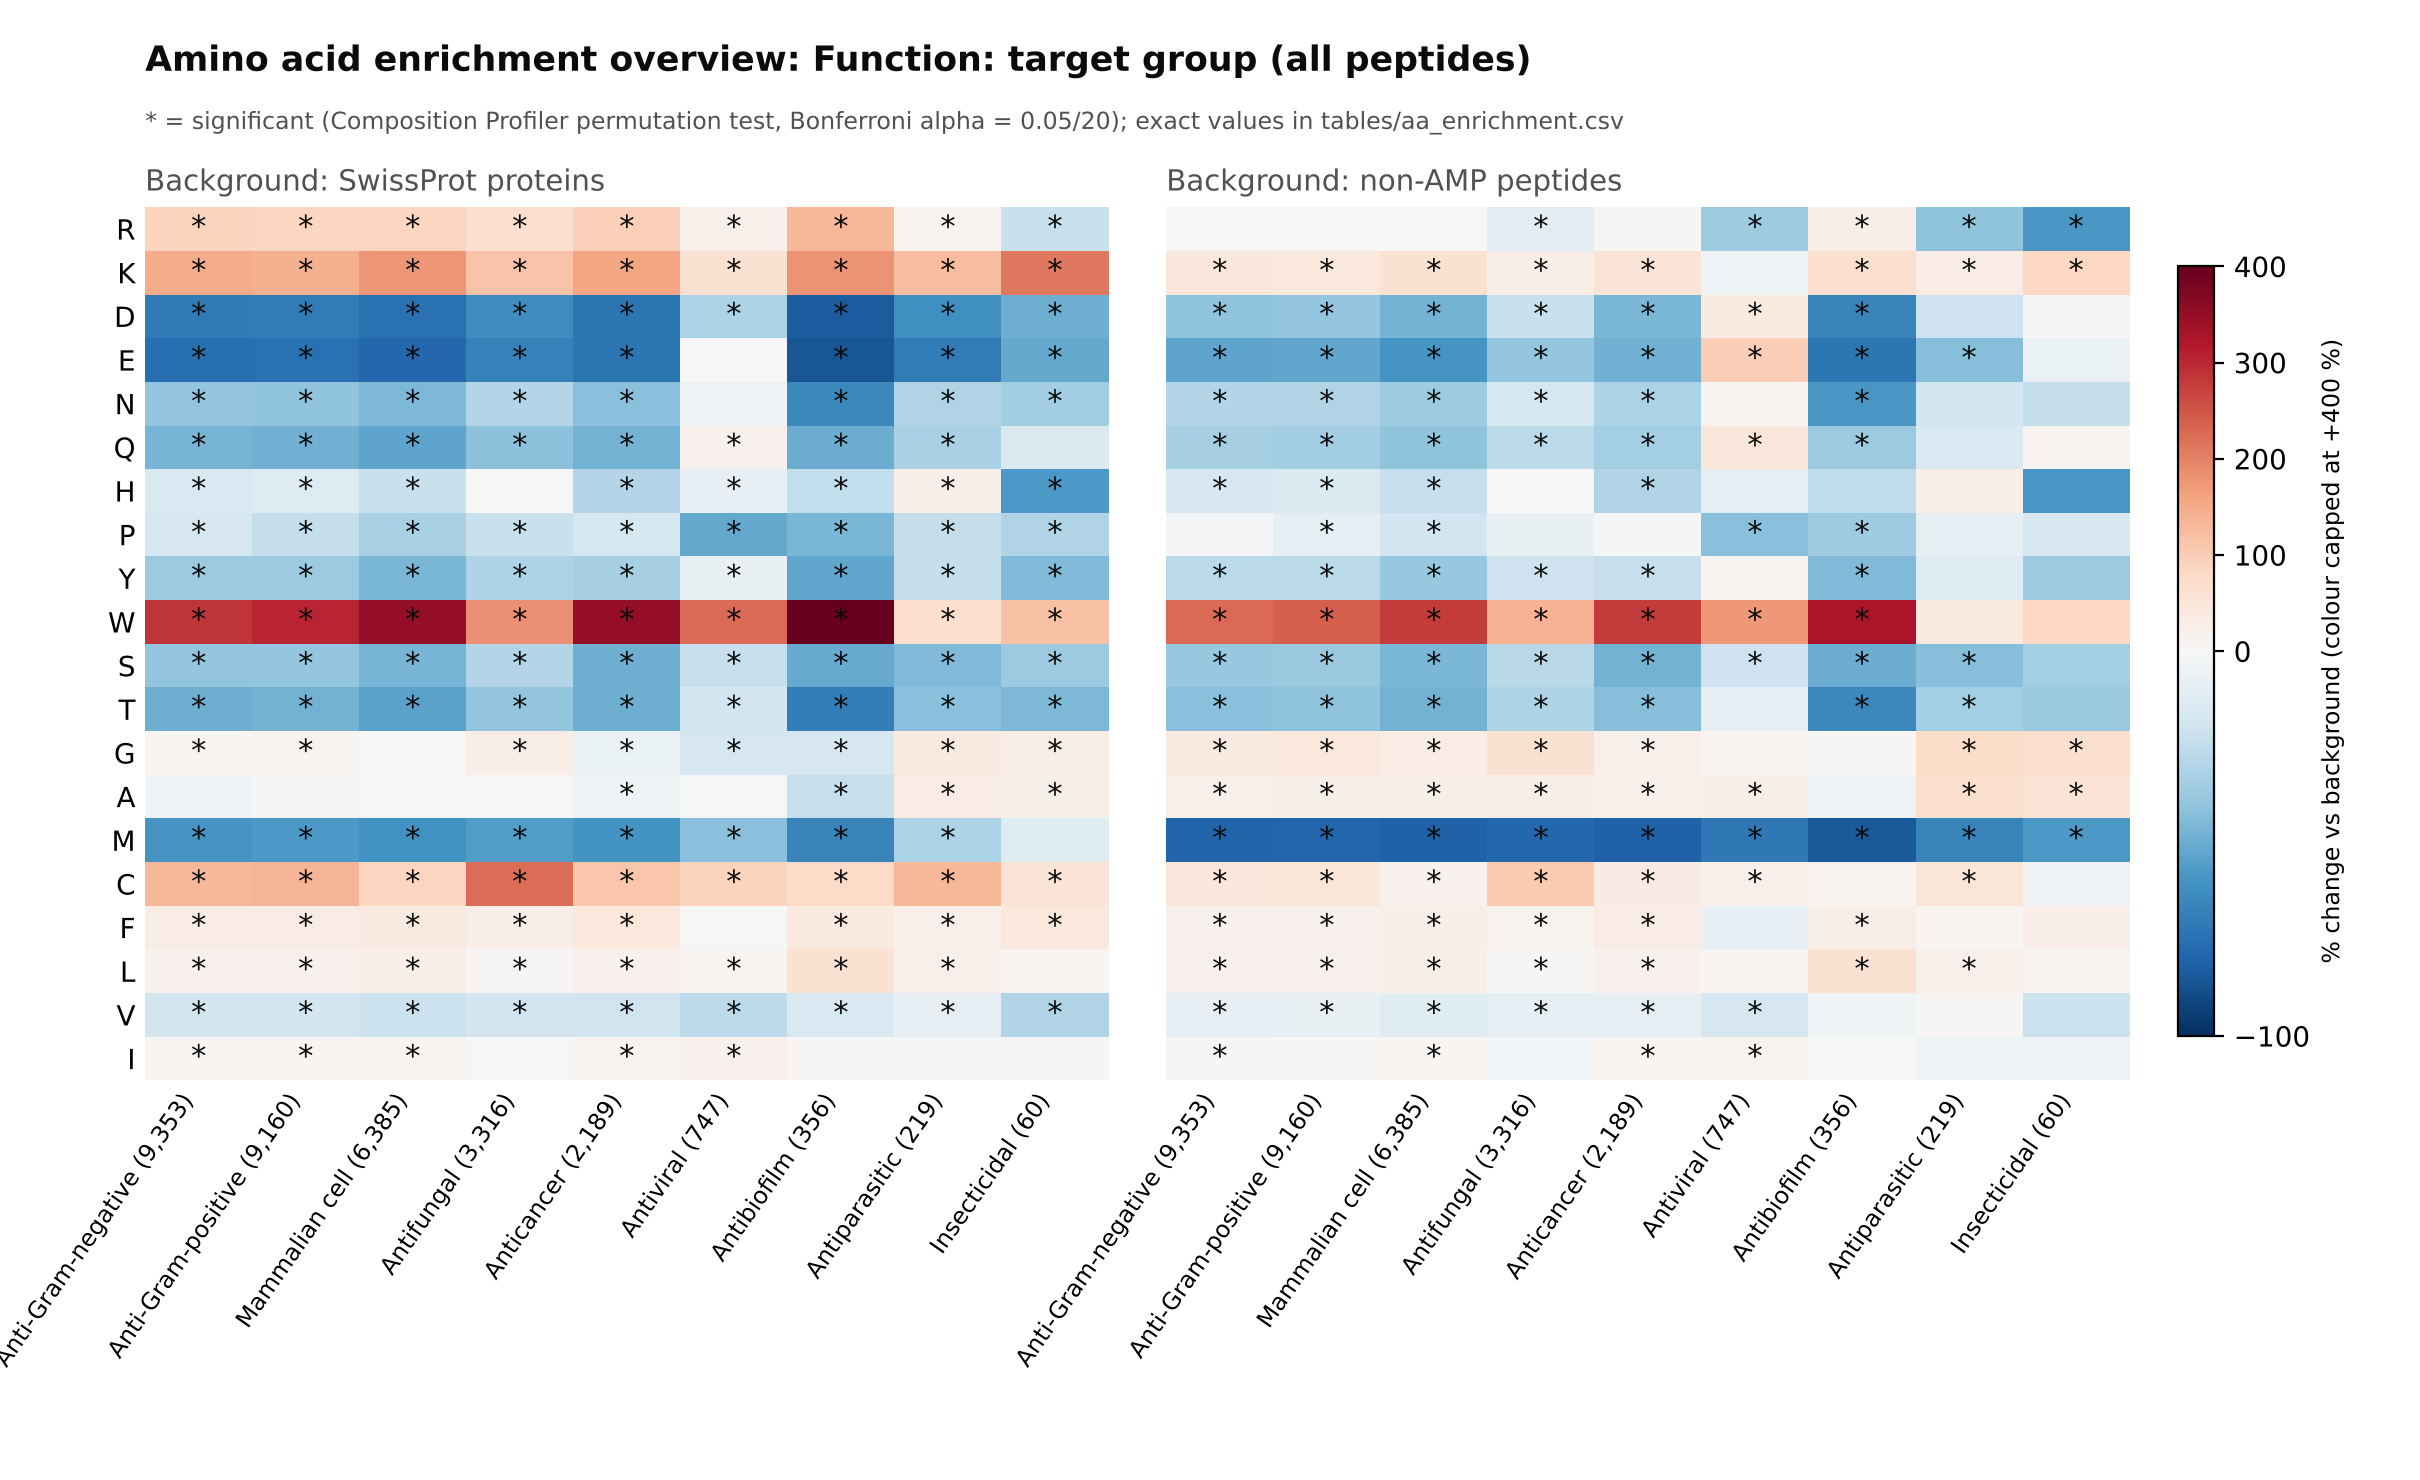
\includegraphics[width=\textwidth]{class_comparisons/function_all/figures/enrichment_heatmap.png}
\caption{Enrichment by target group, all peptides (dominated by Synthetic peptides).}
\end{figure}
\begin{figure}[H]\centering
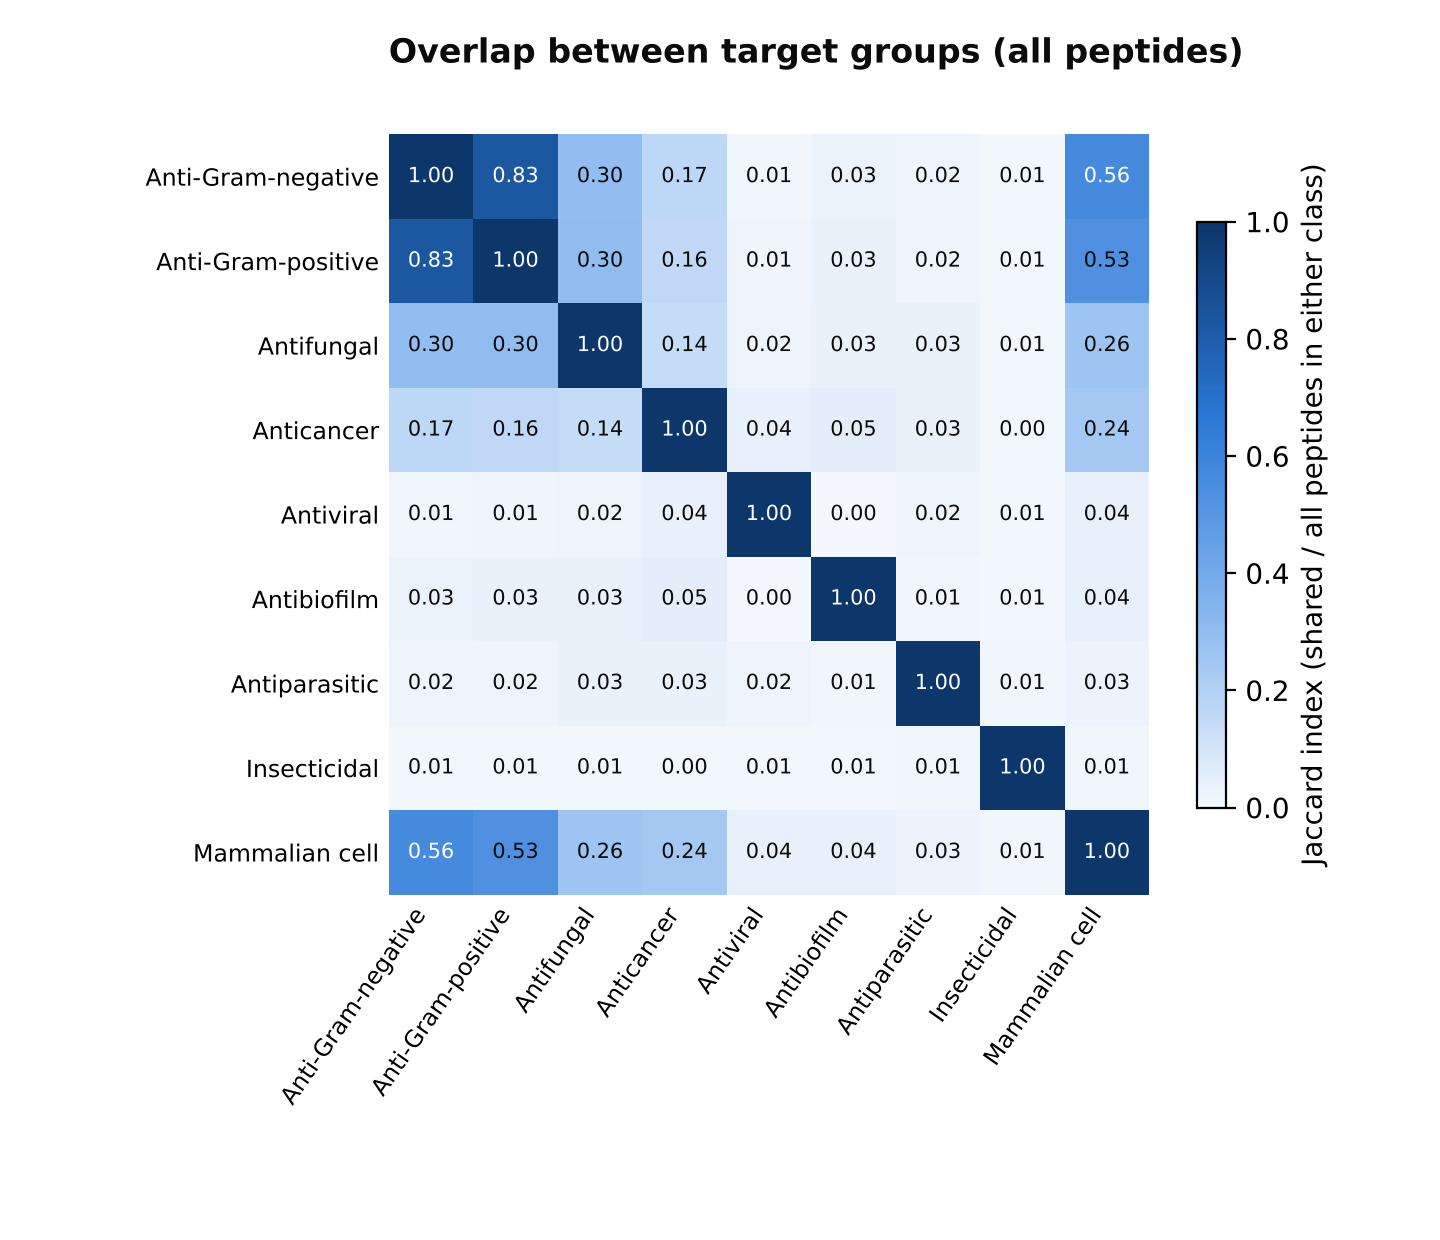
\includegraphics[width=0.55\textwidth]{class_comparisons/overview/figures/function_overlap.png}
\caption{Overlap between target groups (Jaccard index).}
\end{figure}
\begin{figure}[H]\centering
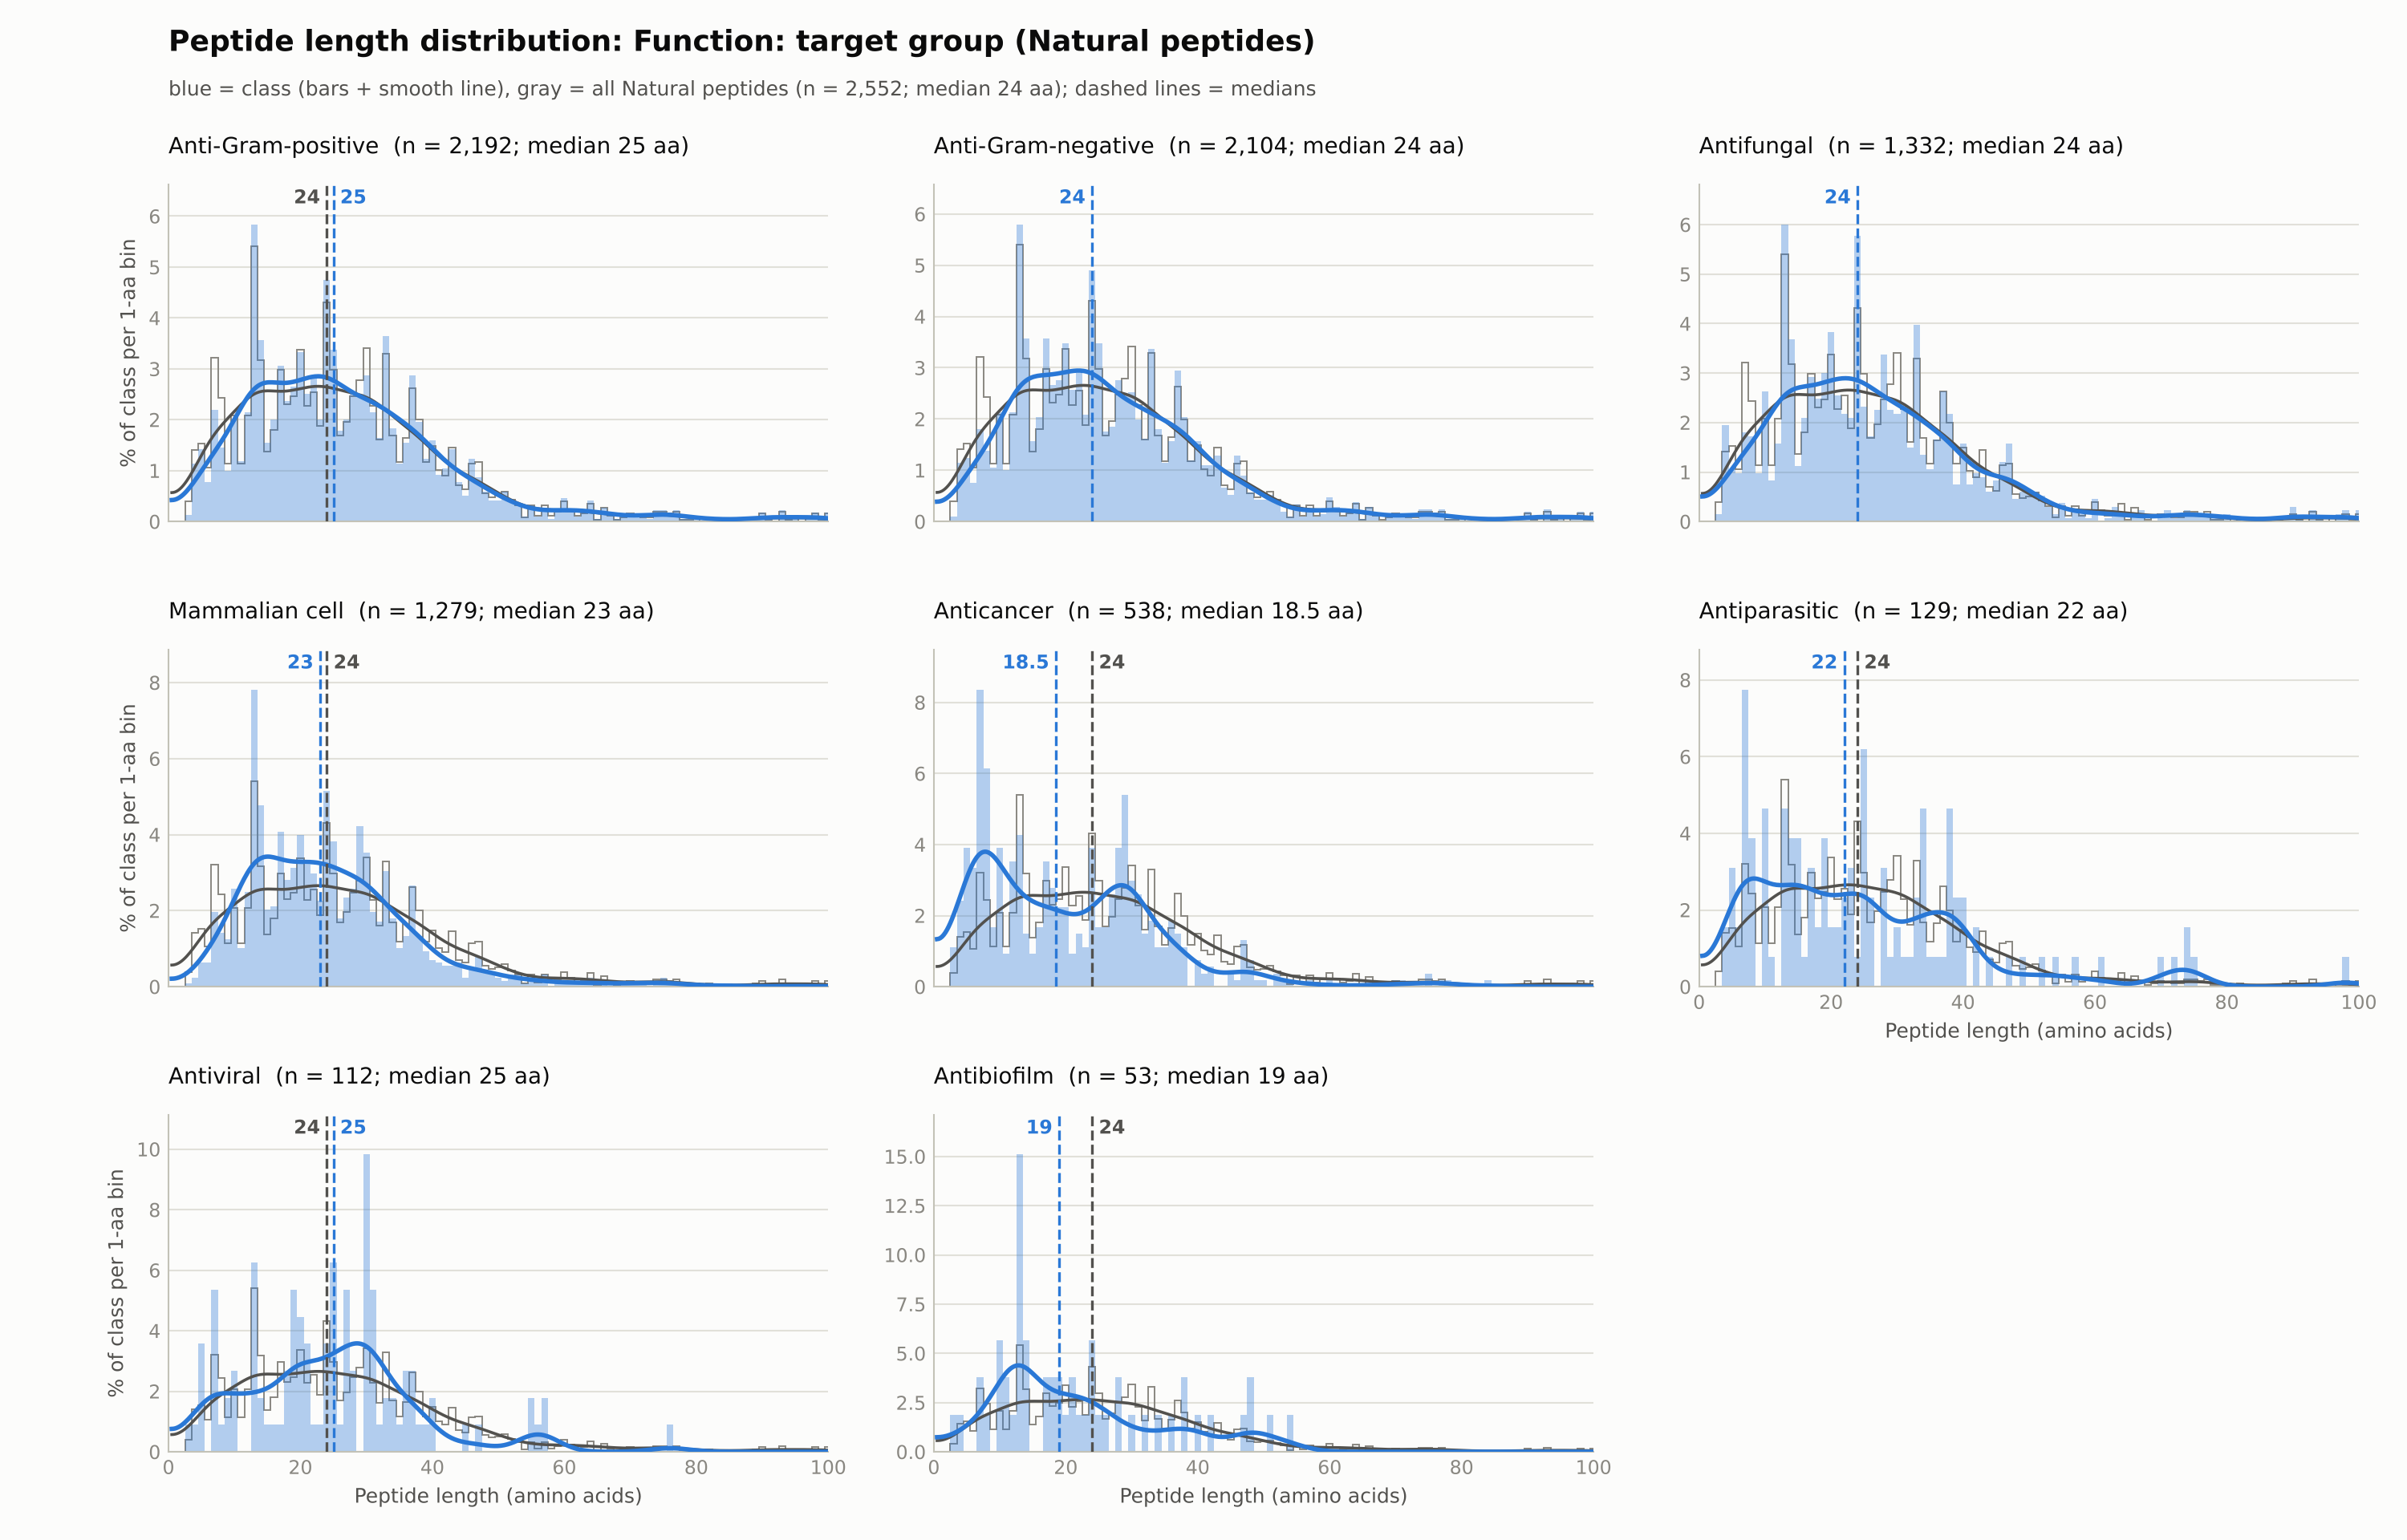
\includegraphics[width=0.95\textwidth]{class_comparisons/function_natural/figures/length_histogram_overlap.png}
\caption{Length of Natural peptides by target group (blue) against all Natural peptides (grey).}
\end{figure}
\begin{itemize}
\item \textbf{All peptides}: every class shows the synthetic pattern (Trp $+64$ to $+405$\,\%, Lys $+62$ to $+210$\,\%, Cys up; Glu, Asp, Met, Thr, Gln down). \textbf{Antiviral} is the exception:
      Glu and Gln are not depleted (vs non-AMP Glu $+97$\,\%), Pro is down ($-51$\,\%).
\item \textbf{Natural only}: all classes share the natural signature (Cys $+88$ to $+531$\,\%, Gly $+38$ to $+58$\,\%). \textbf{Within natural peptides composition follows source, not function.}
      Smaller differences: antiviral natural peptides are the most Cys-rich ($+531$\,\%); mammalian-cell-tested ones have more Lys ($+89$\,\%) and Trp; anticancer ones more Pro, Phe and Ile and less His;
      antibiofilm ($n=53$) the weakest Cys signal.
\item \textbf{Length}: function classes differ little (all peptides: medians 13--18\amin; insecticidal 24.5 and antiparasitic 20 longer). Among Natural peptides, anticancer peptides are shorter
      (18.5 vs 25\amin, $r=-0.30$) and mammalian-cell-tested slightly shorter ($r=-0.14$).
\end{itemize}

\subsection{Target object (mechanism)}
\begin{figure}[H]\centering
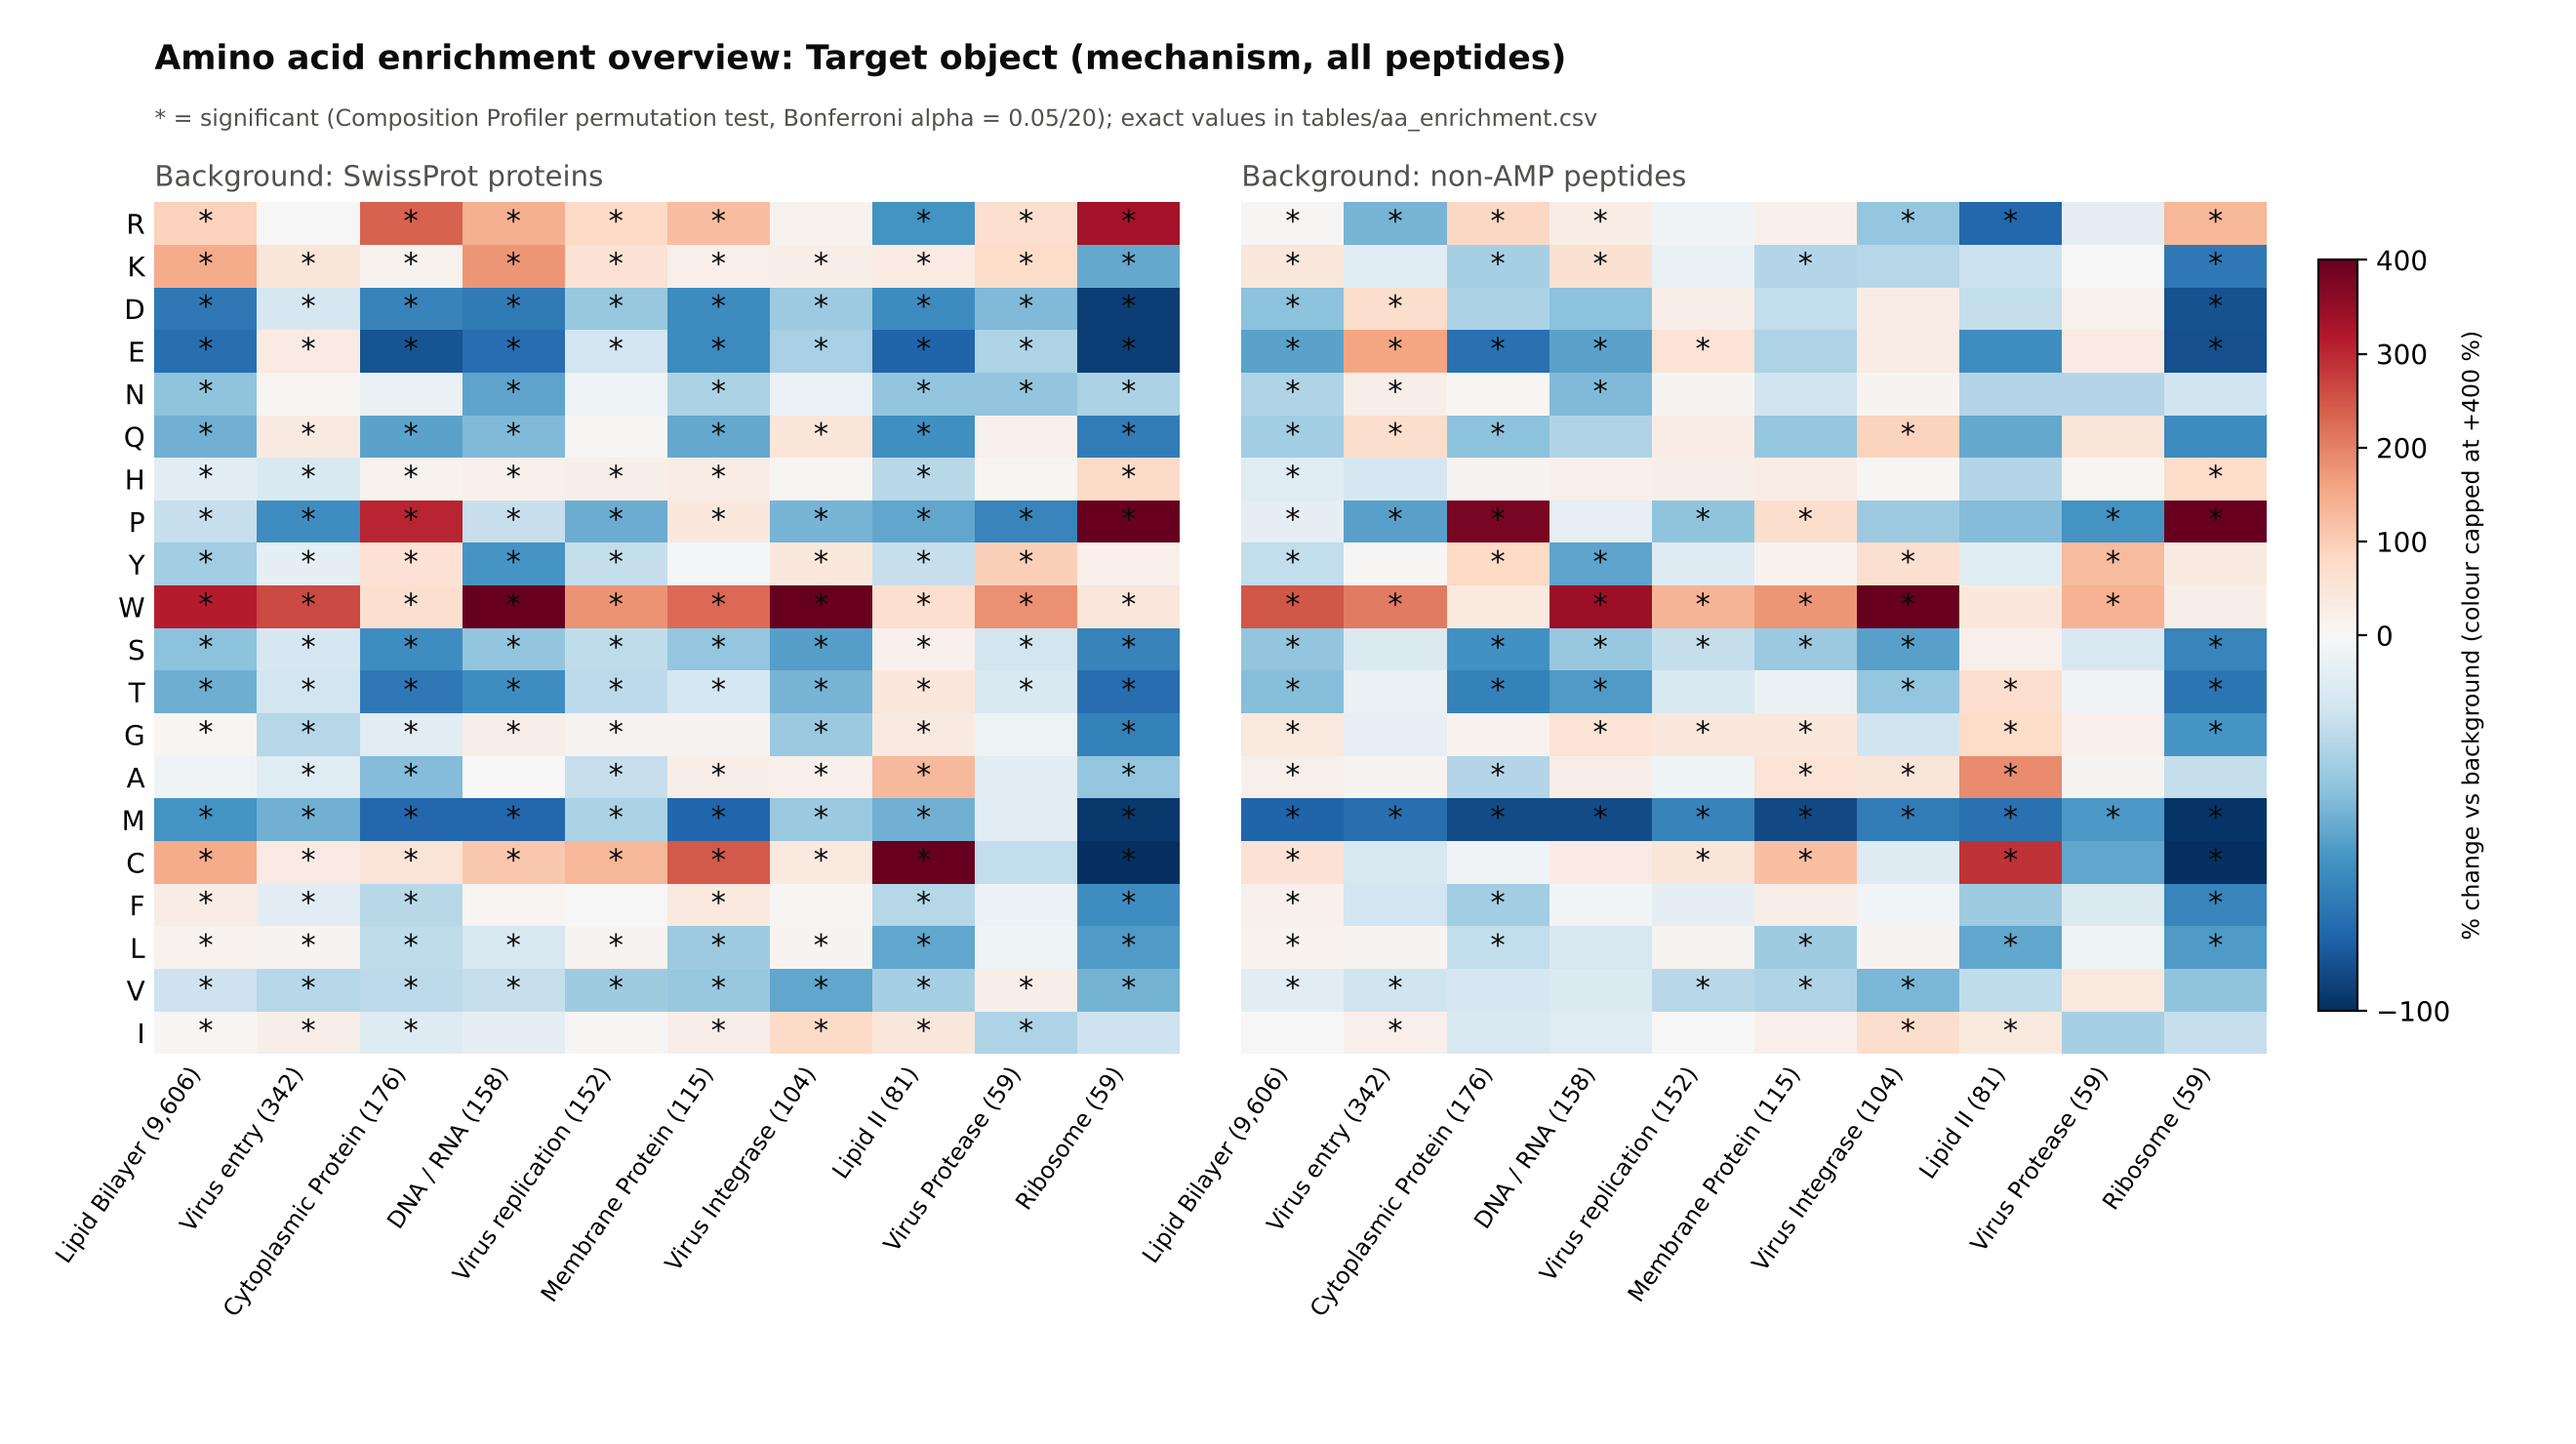
\includegraphics[width=\textwidth]{class_comparisons/target_object/figures/enrichment_heatmap.png}
\caption{Enrichment by target object.}
\end{figure}
\begin{figure}[H]\centering
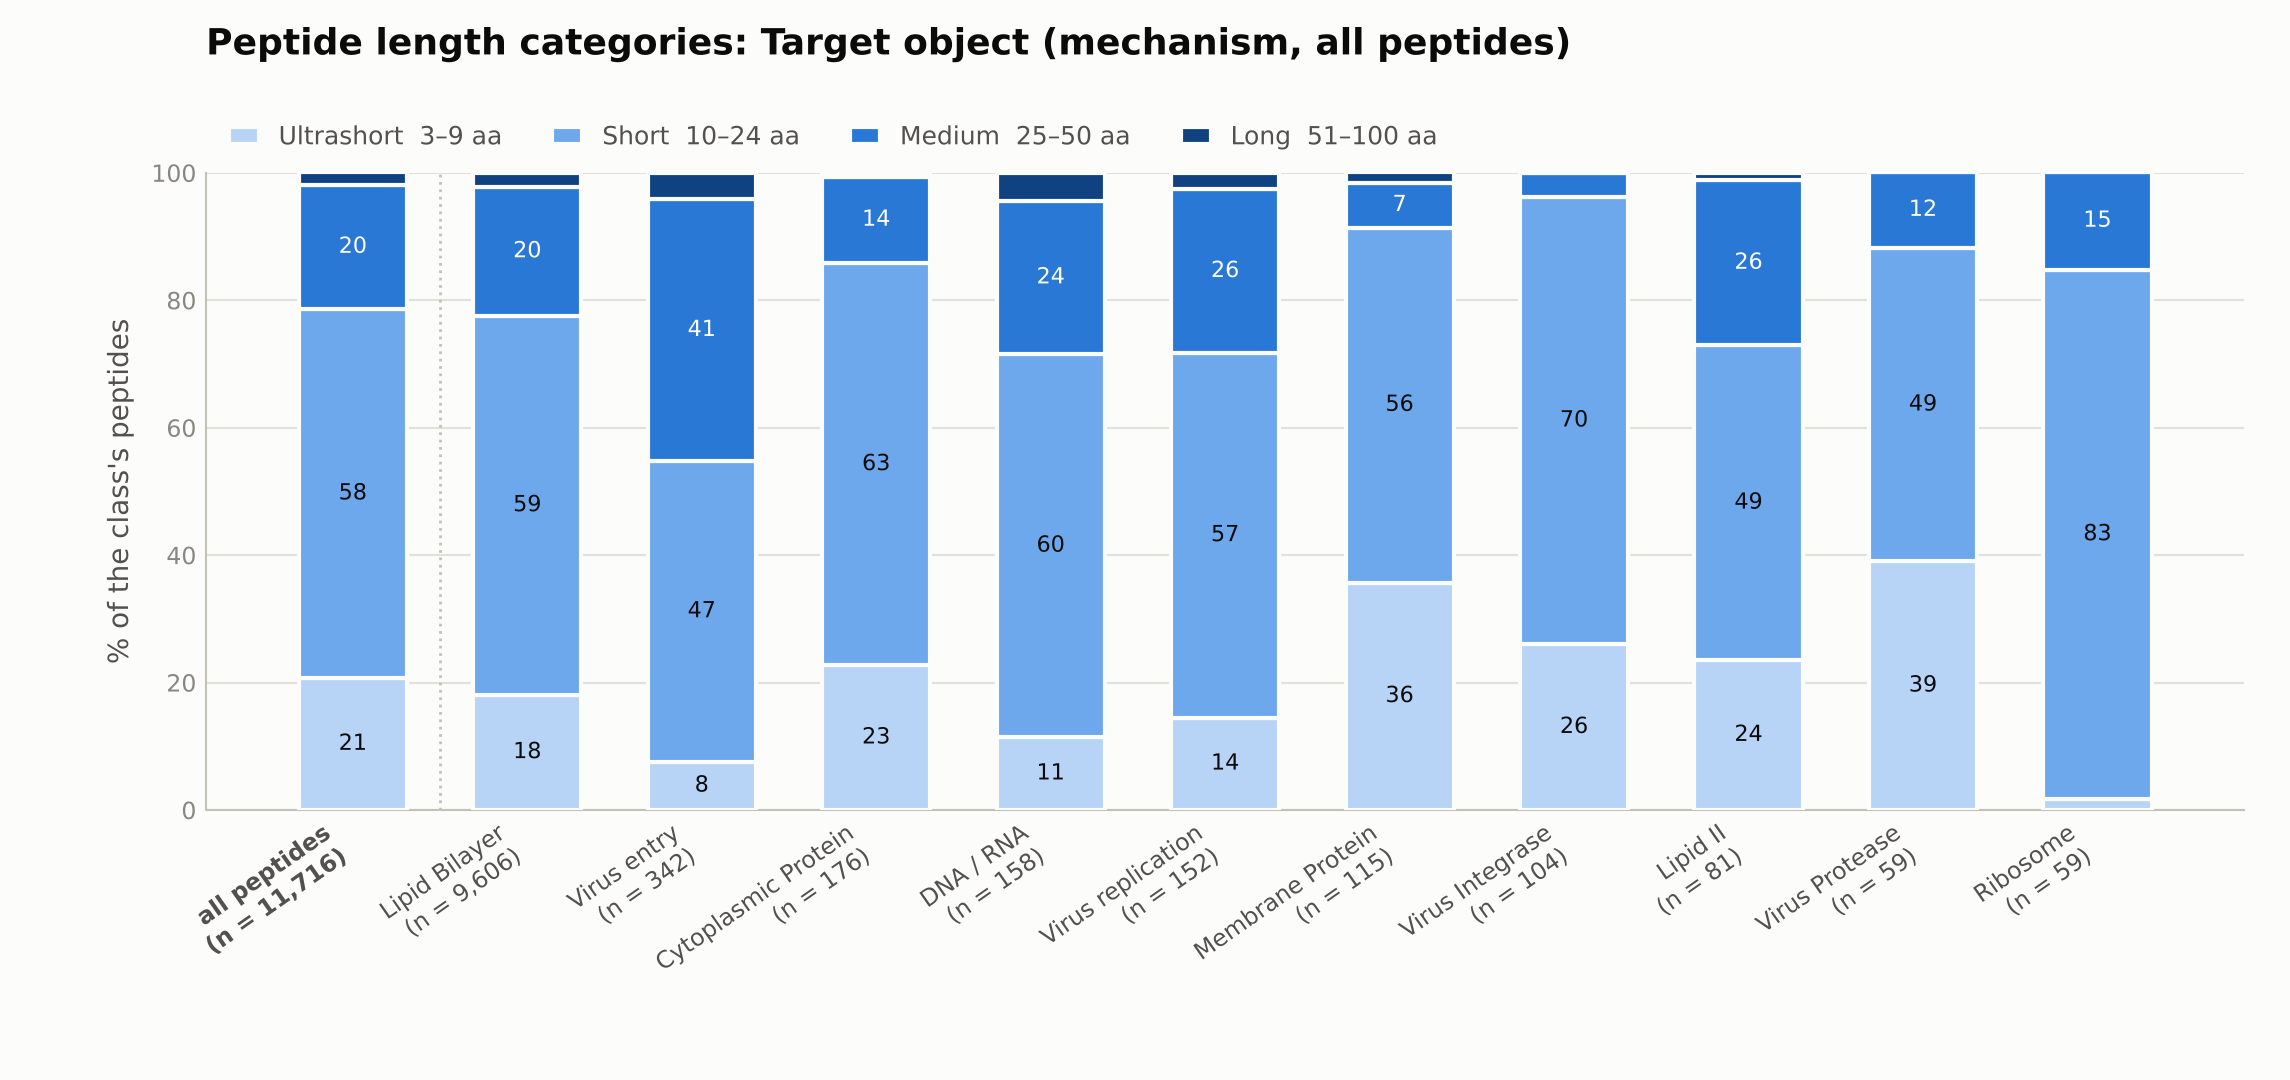
\includegraphics[width=0.8\textwidth]{class_comparisons/target_object/figures/length_category_fraction_bar.png}
\caption{Length categories by target object.}
\end{figure}
\begin{itemize}
\item \textbf{Ribosome} (59) and \textbf{cytoplasmic protein} (176): \textbf{Pro/Arg-rich, Cys-free} (Ribosome: Pro $+625$\,\%, Arg $+333$\,\%, Cys $-100$\,\%, His $+77$\,\%; cytoplasmic protein: Pro $+303$\,\%, Arg $+237$\,\%).
      This is the proline-rich AMP family that enters bacteria and binds the ribosome (or DnaK) instead of lysing the membrane \cite{graf2017}. Ribosome binders are mostly 10--24\amin{} (83\,\%).
\item \textbf{Lipid II} (81): Cys $+514$\,\%, Thr $+47$\,\%, Ile $+44$\,\%; Arg $-59$\,\%, Pro $-52$\,\%, Leu $-52$\,\%; consistent with lantibiotics and defensin-like Lipid II binders \cite{breukink2006}.
      Its Ala $+130$\,\% is mostly former \texttt{X} (lanthionines).
\item \textbf{Virus entry} (342): Trp $+265$\,\% but Glu $+34$\,\% and Gln $+37$\,\% (vs non-AMP Glu $+156$\,\%), Pro $-62$\,\%: anionic peptides, consistent with fusion-protein-derived entry inhibitors;
      longest class (median 21\amin, $r=+0.41$). Virus replication is similar but weaker.
\item \textbf{Virus integrase} (104): Trp $+543$\,\%, Ile, Gln up; short (median 11\amin, $r=-0.36$). \textbf{DNA/RNA} (158): Trp $+425$\,\%, Lys $+175$\,\%, Arg $+142$\,\%.
\item \textbf{Lipid bilayer} (82\,\% of all peptides) reproduces the overall pattern.
\end{itemize}

\subsection{Overview of length}
\begin{figure}[H]\centering
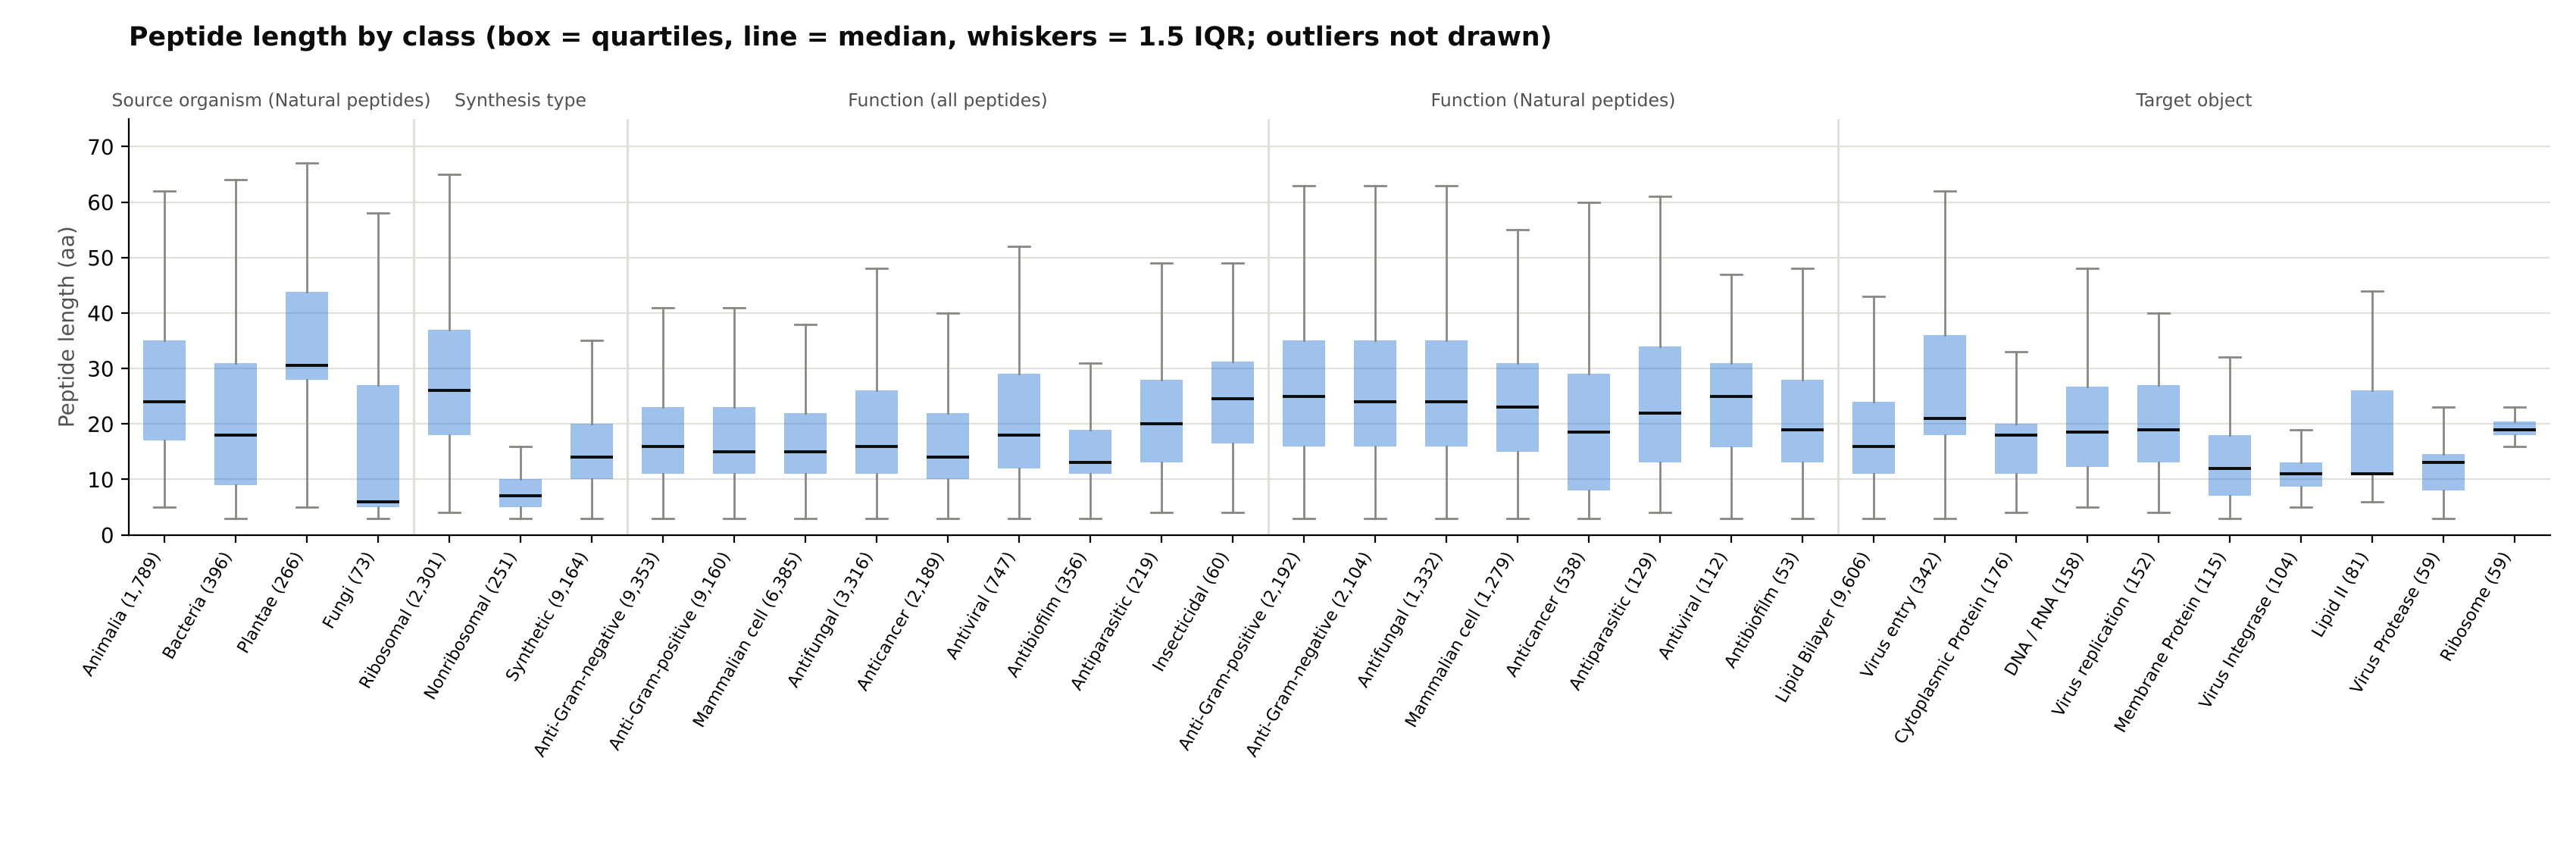
\includegraphics[width=\textwidth]{class_comparisons/overview/figures/length_boxplots.png}
\caption{Length of every tested class.}
\end{figure}

\begin{keypoint}[What the class comparisons add]
(1) The natural Cys/Gly signature belongs to ribosomal peptides and is strongest in plants and fungi; nonribosomal peptides are short, Pro/aromatic-rich and not cationic.
(2) Within natural peptides, target group hardly changes composition; source does. (3) Mechanism does: intracellular binders are Pro/Arg-rich and Cys-free,
virus-entry peptides are anionic, membrane-active peptides follow the cationic AMP pattern.
\end{keypoint}

%======================================================================
\section{Decision log}
%======================================================================
\begin{longtable}{>{\raggedright}p{4.2cm}>{\raggedright}p{4.2cm}>{\raggedright\arraybackslash}p{6.0cm}}
\toprule
Decision & Alternative & Reason\\\midrule\endhead
Natural = Ribosomal + Nonribosomal & Ribosomal only & The only origin field; shown separately in the synthesis-type comparison.\\
Kingdom by \texttt{ID} & by name & Names not unique, inconsistent spacing.\\
Rebuild subsets with a script & re-run notebook by hand & Reproducible; checked to reproduce the notebook's output.\\
Remove multi-chain entries & split chains & Lengths wrong; complexes not comparable.\\
$\geq3$ real residues, $\leq100$\amin & keep all & No composition signal / antimicrobial proteins (APD).\\
\texttt{X} $\geq30$\,\% out, else \texttt{X}$\rightarrow$Ala & drop all / keep \texttt{X} & Keeps length; limits invention. Inflates Ala (reported per class).\\
D-amino acids as L & separate & 20-letter alphabet; chirality affects stability, not composition.\\
CD-HIT 90\,\%, combined & 80\,\%, per origin & Removes near-identical analogues and cross-origin copies; medians unchanged either way.\\
$<10$\amin{} not clustered & cluster 5--9\amin & Cannot reach 90\,\%; would remove 512 exact fragments.\\
\texttt{-l 9}, \texttt{-T 1} & defaults & Default drops 10-aa peptides; single thread reproducible.\\
One peptide set for all comparisons & re-cluster each class & Numbers comparable across comparisons; matches the deliverables.\\
Composition Profiler, official tool & $\chi^2$ on residues & Permutes whole sequences (residues within a peptide are not independent).\\
Two backgrounds & SwissProt only & ``vs proteins'' and ``vs peptides'' are different questions.\\
20 residues, no groups; Bonferroni & groups; FDR & Groups not independent; simple and conservative.\\
$n\geq50$ per tested class & any $n$ & Composition of a few peptides is unstable.\\
Function for all and Natural only & all only & Synthetic dominance hides function signal.\\
Lipid II added as target object & notebook's 23 objects & A real mechanism class with 81 peptides.\\
Small multiples for class histograms & overlapping colours & Up to 10 classes exceed a colour-blind-safe palette; one hue per panel, population in grey.\\
Cut bars above $+5$ & full height & Plant Cys ($+9.4$) would flatten every other bar; value written in the bar.\\
First pass removed & keep & Superseded; had the \texttt{-l} problem and the incomplete export.\\\bottomrule
\end{longtable}

%======================================================================
\section{Limitations and threats to validity}
%======================================================================
\begin{enumerate}
\item \textbf{Annotation semantics}: target groups mean ``tested against'', not ``potent against''; no MIC thresholds.
\item \textbf{Kingdom only for Natural peptides}; 21 Natural peptides unclassified.
\item \textbf{Backgrounds}: old SwissProt sample; non-AMP set not audited; results against it depend on its construction.
\item \textbf{No length adjustment}: classes differ in length; residues are pooled.
\item \textbf{\texttt{X}$\rightarrow$Ala} inflates Ala, strongly in nonribosomal and Lipid II peptides.
\item \textbf{D-amino acids and terminal modifications ignored} in composition.
\item \textbf{CD-HIT greediness and threshold}: slightly different sets with other orders or cut-offs; short fragments not clustered.
\item \textbf{Overlapping classes}: function and target-object classes share peptides; heatmap columns are not independent experiments.
\item \textbf{Small classes}: Fungi (73), antibiofilm-Natural (53), insecticidal (60), ribosome and virus protease (59) are indicative.
\item \textbf{Database bias}: DBAASP reflects what researchers chose to make and test; patterns describe the database, not all AMPs.
\item \textbf{Associations, not causes.}
\item \textbf{Snapshot}: the export is of 2026; DBAASP grows continuously.
\end{enumerate}

%======================================================================
\section{Questions you should be able to answer}
%======================================================================
\begin{description}
\item[Why remove redundancy?] Synthetic libraries are analogue series; 41\,\% of cleaned Synthetic peptides were redundant at 90\,\% identity.
\item[Why 90\,\%?] One substitution in a 10--20-mer gives 90--95\,\% identity, so near-copies are removed while different peptides stay.
\item[Why are peptides under 10\amin{} not clustered?] Different peptides of $\leq9$ residues cannot reach 90\,\%; identical ones are removed as duplicates.
\item[What was the CD-HIT pitfall?] Default \texttt{-l 10} silently discards 10-aa sequences; fixed with \texttt{-l 9} and a count check.
\item[What was wrong with the first export?] One page was downloaded twice, so 2{,}000 entries were missing. Fixed: 11{,}716 instead of 10{,}824 peptides, same conclusions.
\item[Why two backgrounds?] Proteins vs peptides: the non-AMP comparison shows that charge alone is not AMP-specific.
\item[Why is Cys enriched in Natural peptides?] Disulfide-stabilised families (defensins, thionins, cyclotides), especially in plants and fungi.
\item[Why is Trp enriched in Synthetic peptides?] Trp anchors peptides at the membrane interface and is a design favourite.
\item[Does function determine composition?] Within Natural peptides hardly; source and mechanism do.
\item[Why are ribosome-targeting peptides different?] They are proline-rich AMPs that enter the cell and bind the ribosome: Pro/Arg-rich, no Cys.
\item[Why can't the Ala result of nonribosomal peptides be trusted?] One residue in ten was \texttt{X} and became Ala in cleaning.
\item[Why are the class histograms drawn as panels?] Up to 10 classes cannot be told apart in one overlaid plot; each panel compares one class with the population.
\item[Weakest parts?] Unaudited non-AMP background, ``tested against'' function labels, no length adjustment.
\end{description}

%======================================================================
\section{Reproducing the work}
%======================================================================
\begin{verbatim}
pip install -r requirements.txt     # pandas numpy matplotlib scipy openpyxl
sudo apt-get install cd-hit                   # tested with 4.8.1
git clone https://github.com/vvacic/cprofiler && pip install -e cprofiler

python "data collection/build_subsets.py"     # export pages -> raw_data zip
python deliverables/scripts/01_remove_redundancy.py
python deliverables/scripts/02_make_figures.py
python deliverables/scripts/03_check_cdhit_result.py
python deliverables/scripts/04_aa_enrichment.py          # ~1 min
python deliverables/scripts/05_enrichment_figures.py
python deliverables/scripts/06_sequences_lost_xlsx.py
python class_comparisons/scripts/01_build_class_table.py
python class_comparisons/scripts/02_length_figures.py
python class_comparisons/scripts/03_aa_enrichment.py      # ~30 min
python class_comparisons/scripts/04_enrichment_figures.py
python class_comparisons/scripts/05_annotation_shares.py
\end{verbatim}
All random steps use fixed seeds; CD-HIT runs single-threaded; the scripts assert that counts add up and that the class comparisons reproduce the deliverable table.

%======================================================================
\section{Possible next steps}
%======================================================================
\begin{enumerate}
\item Potency-based function classes (e.g.\ MIC $\leq 32\,\mu$g/mL) instead of ``tested against''.
\item Length-matched comparisons (e.g.\ within the Short class) to separate length from origin.
\item A current, full SwissProt background and an audited, length-matched non-AMP background.
\item Physicochemical descriptors (net charge, hydrophobic moment) per class.
\item Treat non-standard residues explicitly (ornithine, lanthionine) instead of \texttt{X}$\rightarrow$Ala, at least for nonribosomal and Lipid II peptides.
\item An automated, timed pipeline from download to figures (``Option~2'').
\end{enumerate}

%======================================================================
\appendix
\section{File guide}
%======================================================================
\begin{longtable}{>{\raggedright}p{6.6cm}>{\raggedright\arraybackslash}p{7.9cm}}
\toprule File & Content\\\midrule\endhead
\texttt{data collection/build\_subsets.py} & export pages $\rightarrow$ raw subsets\\
\file{raw_data/dbaasp_datasets_corrected.zip}, \file{manifest.csv} & raw subsets and their sizes\\
\file{deliverables/fasta/amp_cdhit90.fasta} & final 11{,}716 peptides (+ Natural and Synthetic files)\\
\file{deliverables/tables/removed_records.csv} & every lost record, reason, covering peptide\\
\file{deliverables/tables/aa_enrichment.csv} & Natural/Synthetic enrichment, two backgrounds\\
\file{deliverables/tables/cdhit_checks.csv} & integrity checks and what-ifs\\
\file{deliverables/sequences_lost.xlsx} & loss table with explanations\\
\file{class_comparisons/overview/tables/class_peptides.csv} & every peptide with all class labels\\
\file{class_comparisons/overview/tables/class_sizes.csv} & every class, n, tested\\
\file{class_comparisons/overview/tables/annotation_shares.csv} & modifications, D-aa, X, tested targets per class\\
\file{class_comparisons/overview/tables/former_x_share_by_class.csv} & Ala inflation per class\\
\file{class_comparisons/<comparison>/tables/aa_enrichment.csv} & enrichment per class and background\\
\file{class_comparisons/<comparison>/tables/length_*.csv} & length summary, categories, tests\\
\file{class_comparisons/<comparison>/fasta/} & peptides of each class\\\bottomrule
\end{longtable}

\section{Glossary}
\begin{description}[itemsep=1pt]
\item[AMP] antimicrobial peptide. \item[aa] amino acid(s) / residues. \item[D-amino acid] mirror-image residue, lower case in DBAASP. \item[X] non-standard residue.
\item[Ribosomal / Nonribosomal] made by the ribosome / by non-ribosomal peptide synthetases. \item[PrAMP] proline-rich AMP. \item[Lipid II] cell-wall precursor targeted by lantibiotics.
\item[Amidation] C-terminal \texttt{-CONH$_2$}; removes a negative charge. \item[Representative] the sequence CD-HIT keeps for a cluster (the longest).
\item[Fractional difference] (query $-$ background)/background frequency. \item[Bonferroni] divide $\alpha$ by the number of tests.
\item[Rank-biserial $r$] effect size of Mann--Whitney, $-1$ to $+1$. \item[Jaccard] shared / union of two sets.
\end{description}

\begin{thebibliography}{99}\small
\bibitem{zasloff2002} Zasloff M. Antimicrobial peptides of multicellular organisms. \emph{Nature} 415:389--395 (2002). doi:10.1038/415389a
\bibitem{hancock2006} Hancock REW, Sahl HG. Antimicrobial and host-defense peptides as new anti-infective therapeutic strategies. \emph{Nat Biotechnol} 24:1551--1557 (2006). doi:10.1038/nbt1267
\bibitem{ganz2003} Ganz T. Defensins: antimicrobial peptides of innate immunity. \emph{Nat Rev Immunol} 3:710--720 (2003). doi:10.1038/nri1180
\bibitem{chan2006} Chan DI, Prenner EJ, Vogel HJ. Tryptophan- and arginine-rich antimicrobial peptides: structures and mechanisms of action. \emph{Biochim Biophys Acta} 1758:1184--1202 (2006). doi:10.1016/j.bbamem.2006.04.006
\bibitem{graf2017} Graf M, Mardirossian M, Nguyen F, et al. Proline-rich antimicrobial peptides targeting protein synthesis. \emph{Nat Prod Rep} 34:702--711 (2017). doi:10.1039/c7np00020k
\bibitem{breukink2006} Breukink E, de Kruijff B. Lipid II as a target for antibiotics. \emph{Nat Rev Drug Discov} 5:321--332 (2006). doi:10.1038/nrd2004
\bibitem{pirtskhalava2021} Pirtskhalava M, et al. DBAASP v3: database of antimicrobial/cytotoxic activity and structure of peptides as a resource for development of new therapeutics. \emph{Nucleic Acids Res} 49:D288--D297 (2021). doi:10.1093/nar/gkaa991
\bibitem{wang2022} Wang G. Unifying the classification of antimicrobial peptides in the antimicrobial peptide database. \emph{Methods Enzymol} 663:1--18 (2022). doi:10.1016/bs.mie.2021.09.006
\bibitem{li2006} Li W, Godzik A. Cd-hit: a fast program for clustering and comparing large sets of protein or nucleotide sequences. \emph{Bioinformatics} 22:1658--1659 (2006). doi:10.1093/bioinformatics/btl158
\bibitem{fu2012} Fu L, Niu B, Zhu Z, Wu S, Li W. CD-HIT: accelerated for clustering the next-generation sequencing data. \emph{Bioinformatics} 28:3150--3152 (2012). doi:10.1093/bioinformatics/bts565
\bibitem{vacic2007} Vacic V, Uversky VN, Dunker AK, Lonardi S. Composition Profiler: a tool for discovery and visualization of amino acid composition differences. \emph{BMC Bioinformatics} 8:211 (2007). doi:10.1186/1471-2105-8-211
\bibitem{uniprot2023} The UniProt Consortium. UniProt: the Universal Protein Knowledgebase in 2023. \emph{Nucleic Acids Res} 51:D523--D531 (2023). doi:10.1093/nar/gkac1052
\end{thebibliography}

\end{document}
